\begin{enumerate}
\item Your printer has been pre-calibrated and tested, however, after unpacking all of the components you will need to re-mount the Y axis onto the frame and connect the bed and Y axis connectors. You will also need to re-mount the extruder tool head. Please follow the steps completely to make certain that the extruder tool head and Y axis are re-mounted correctly and you will be on your way to your first print.

\item Place the TAZ frame and Y axis assembly on a flat and level surface. Move to the Y axis assembly and find the four Y axis bolts. The four bolts located on the Y axis aluminum frame bars, have large plastic knobs that allow the bolts to be easily turned by hand (Fig. \ref{fig:Y_axis_bolts}, page \pageref{fig:Y_axis_bolts}). Turning counter clock-wise, remove each of the four Y axis bolts and set aside (Fig. \ref{fig:remove_Y_axis_bolts}, page \pageref{fig:remove_Y_axis_bolts}).

\begin{figure}[hp]
\centering
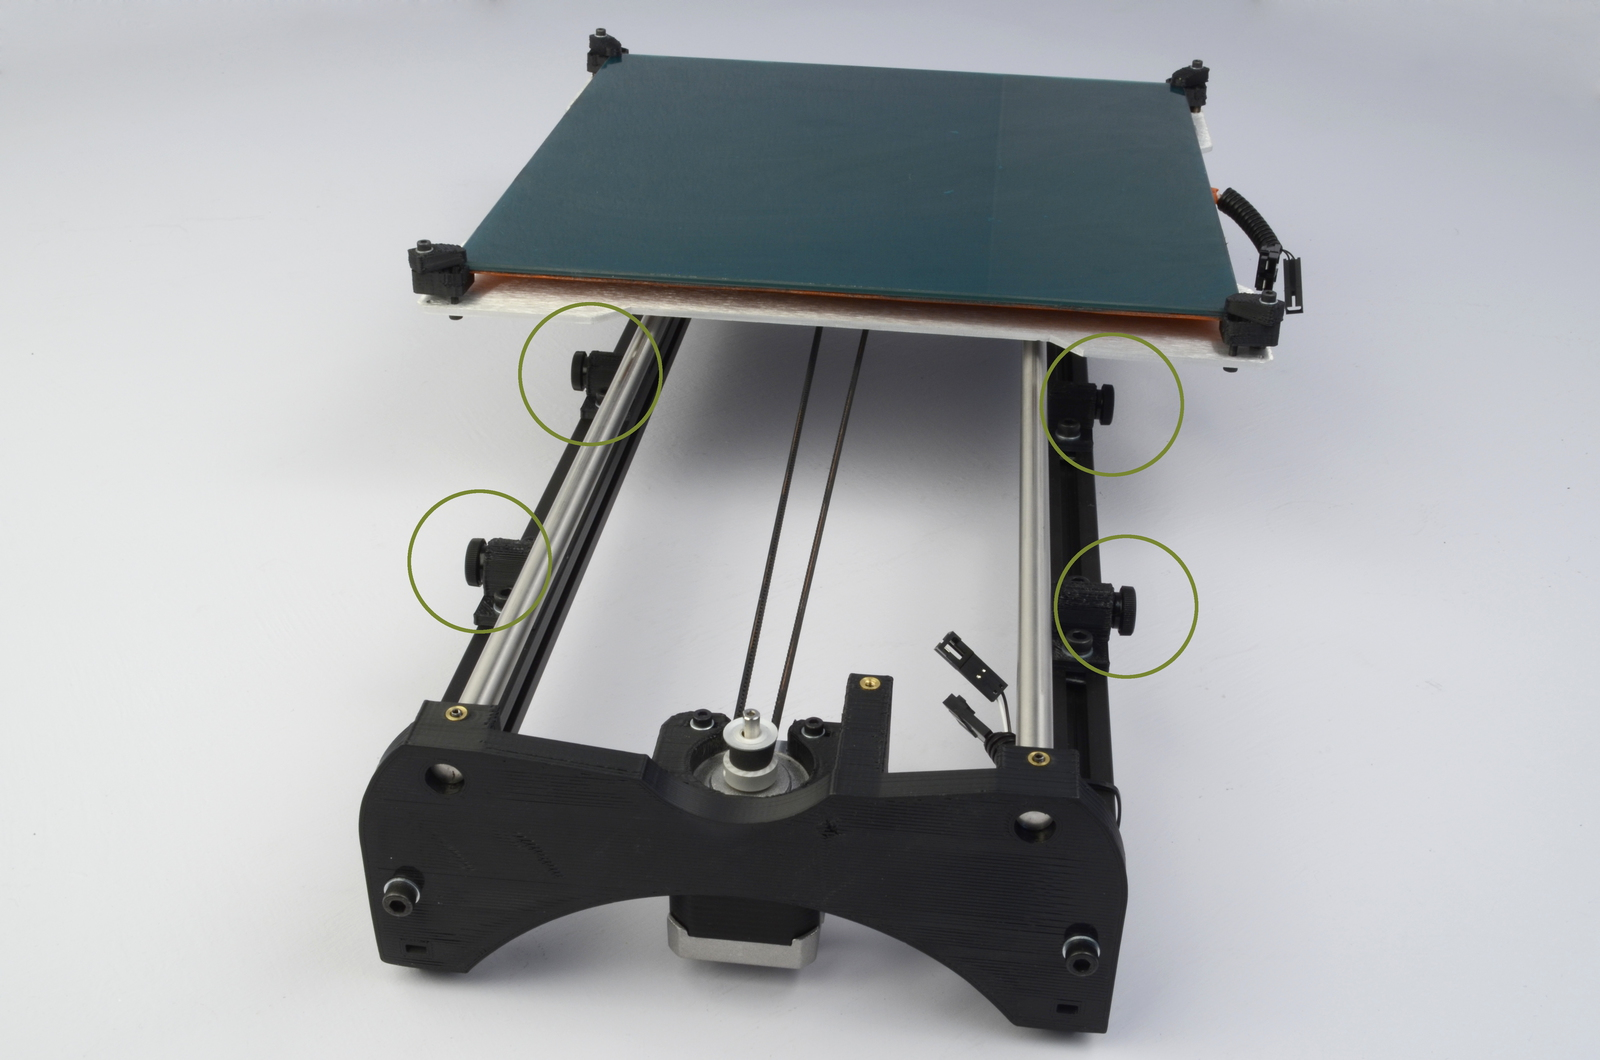
\includegraphics[keepaspectratio=true,angle=0,height=0.4\textheight,width=1.0\textwidth]{y_axis_bolts.JPG}
\caption{Locate the four Y axis bolts}
\label{fig:Y_axis_bolts}
\end{figure}

%\begin{figure}[hp] CD changed to force pic placement
\begin{figure}[H]
\centering
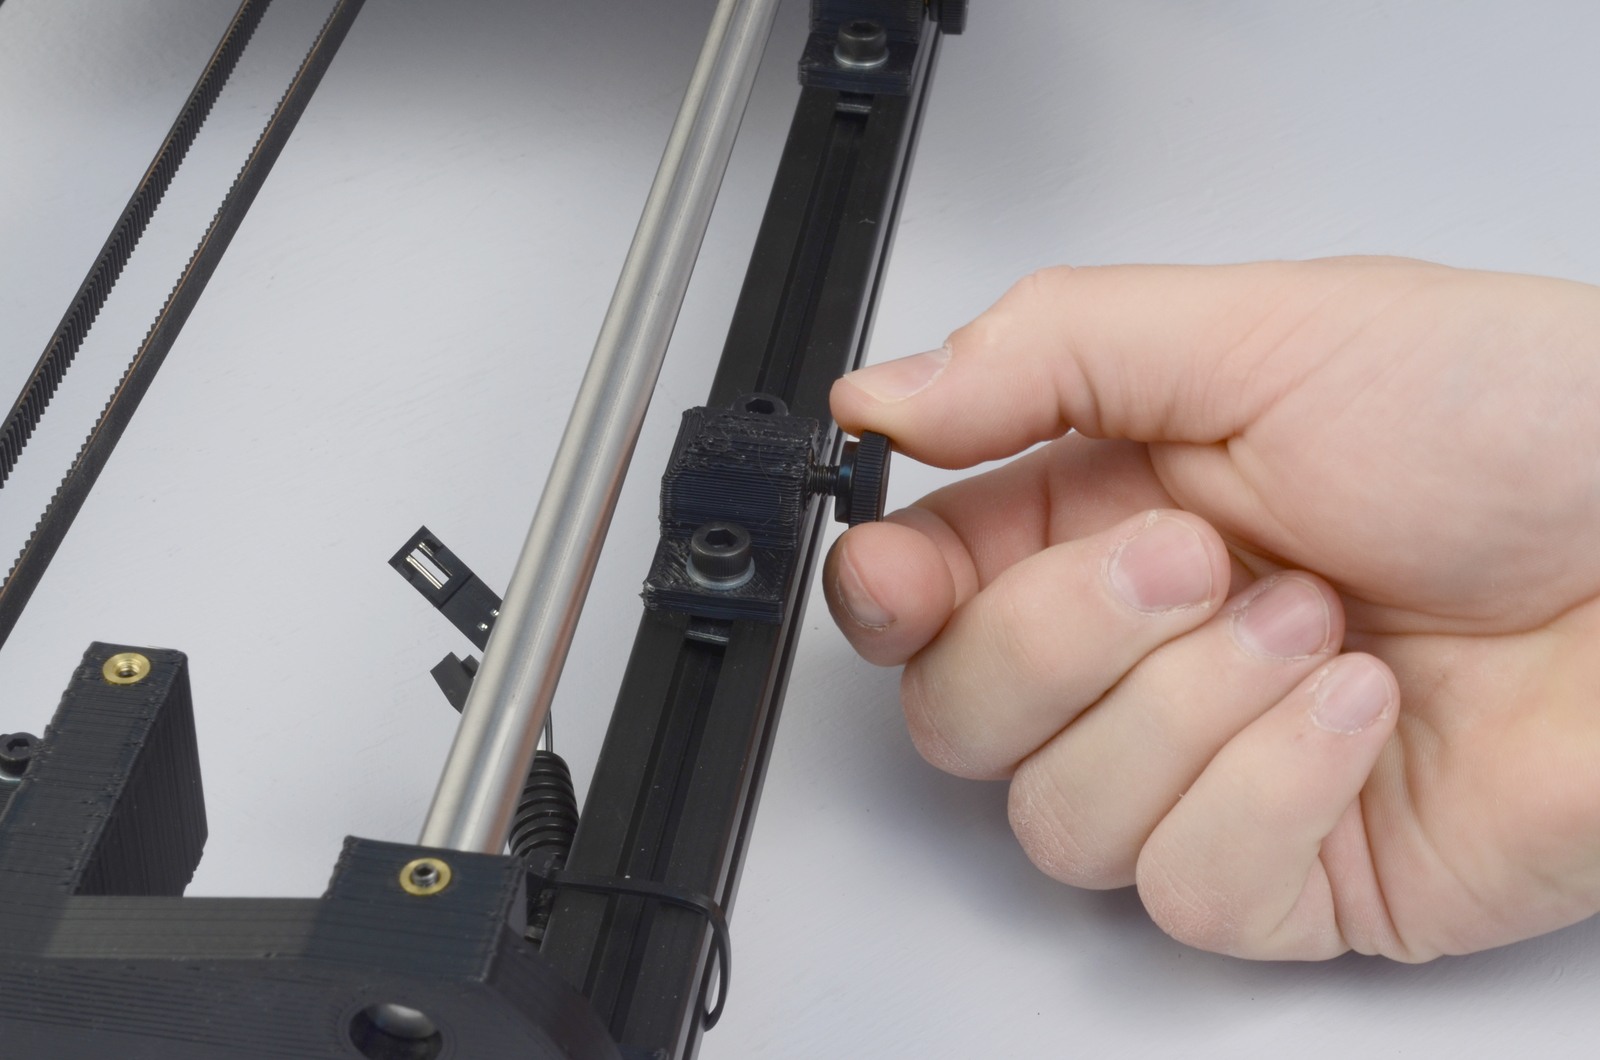
\includegraphics[keepaspectratio=true,angle=0,height=0.4\textheight,width=1.0\textwidth]{y_axis_bolt_remove.JPG}
\caption{Remove the four Y axis bolts}
\label{fig:remove_Y_axis_bolts}
\end{figure}

\item On the TAZ frame locate the four Y axis mount brackets shown in Fig. \ref{fig:frame_Y_axis_mounts} (pg. \pageref{fig:frame_Y_axis_mounts}). With the print surface facing up and the stepper motor end of the Y axis facing back, slide the Y axis assembly in between the Y axis mount brackets. The four Y axis mount brackets will line up with the Y axis bolt holes on the Y axis assembly. Thread the four Y axis bolts through the brackets, into the Y axis assembly (Fig. \ref{fig:Y_axis_bolts_tighten}, page \pageref{fig:Y_axis_bolts_tighten}). Before completely tightening the Y axis bolts make sure the Y axis aluminum bars are pushed down against the TAZ frame lower bars. You can do this by slightly tilting the printer, on the side edge, enough to lift the feet of the Y axis off of the table. The weight of the Y axis will seat it against the TAZ frame. While the printer is slightly tilted tighten the four Y axis bolts. The printer can be now be set flat on the table.
%\begin{figure}[hp] CD forcing image placement
\begin{figure}[H]
\centering
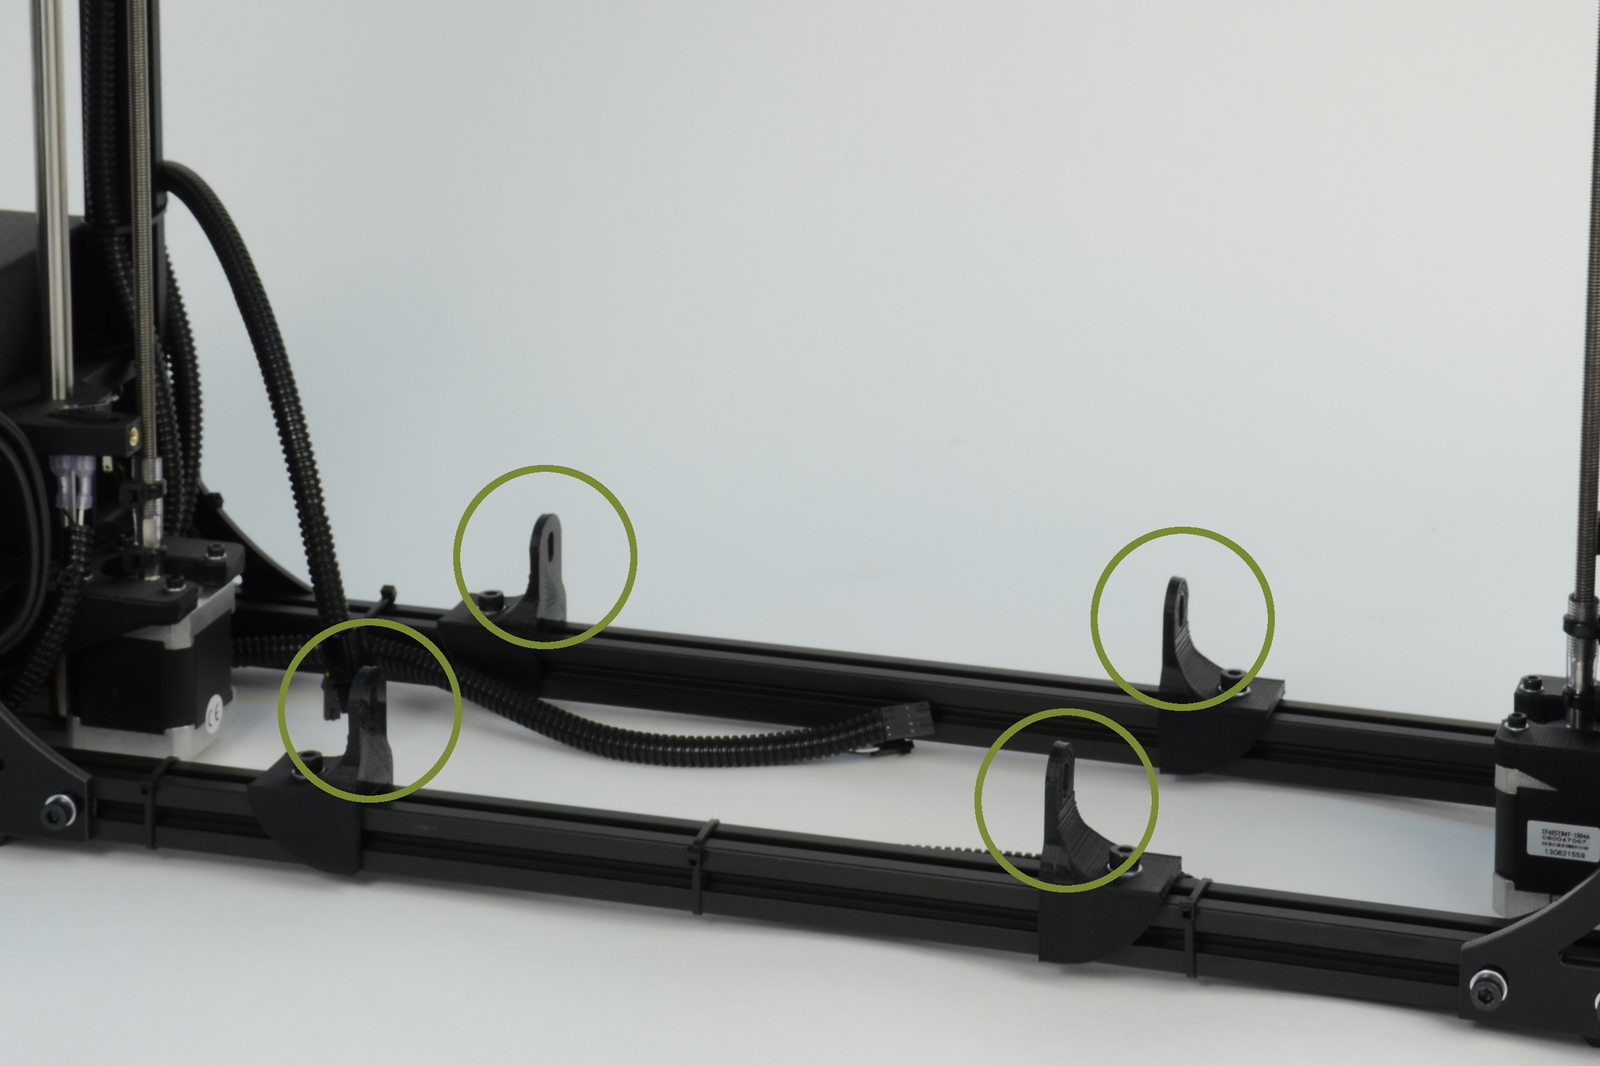
\includegraphics[keepaspectratio=true,angle=0,height=0.4\textheight,width=1.0\textwidth]{frame_y_axis_connector.JPG}
\caption{Locate the four Y axis mounts on the frame}
\label{fig:frame_Y_axis_mounts}
\end{figure}

%\begin{figure}[hp] CD forcing image placement
\begin{figure}[H]
\centering
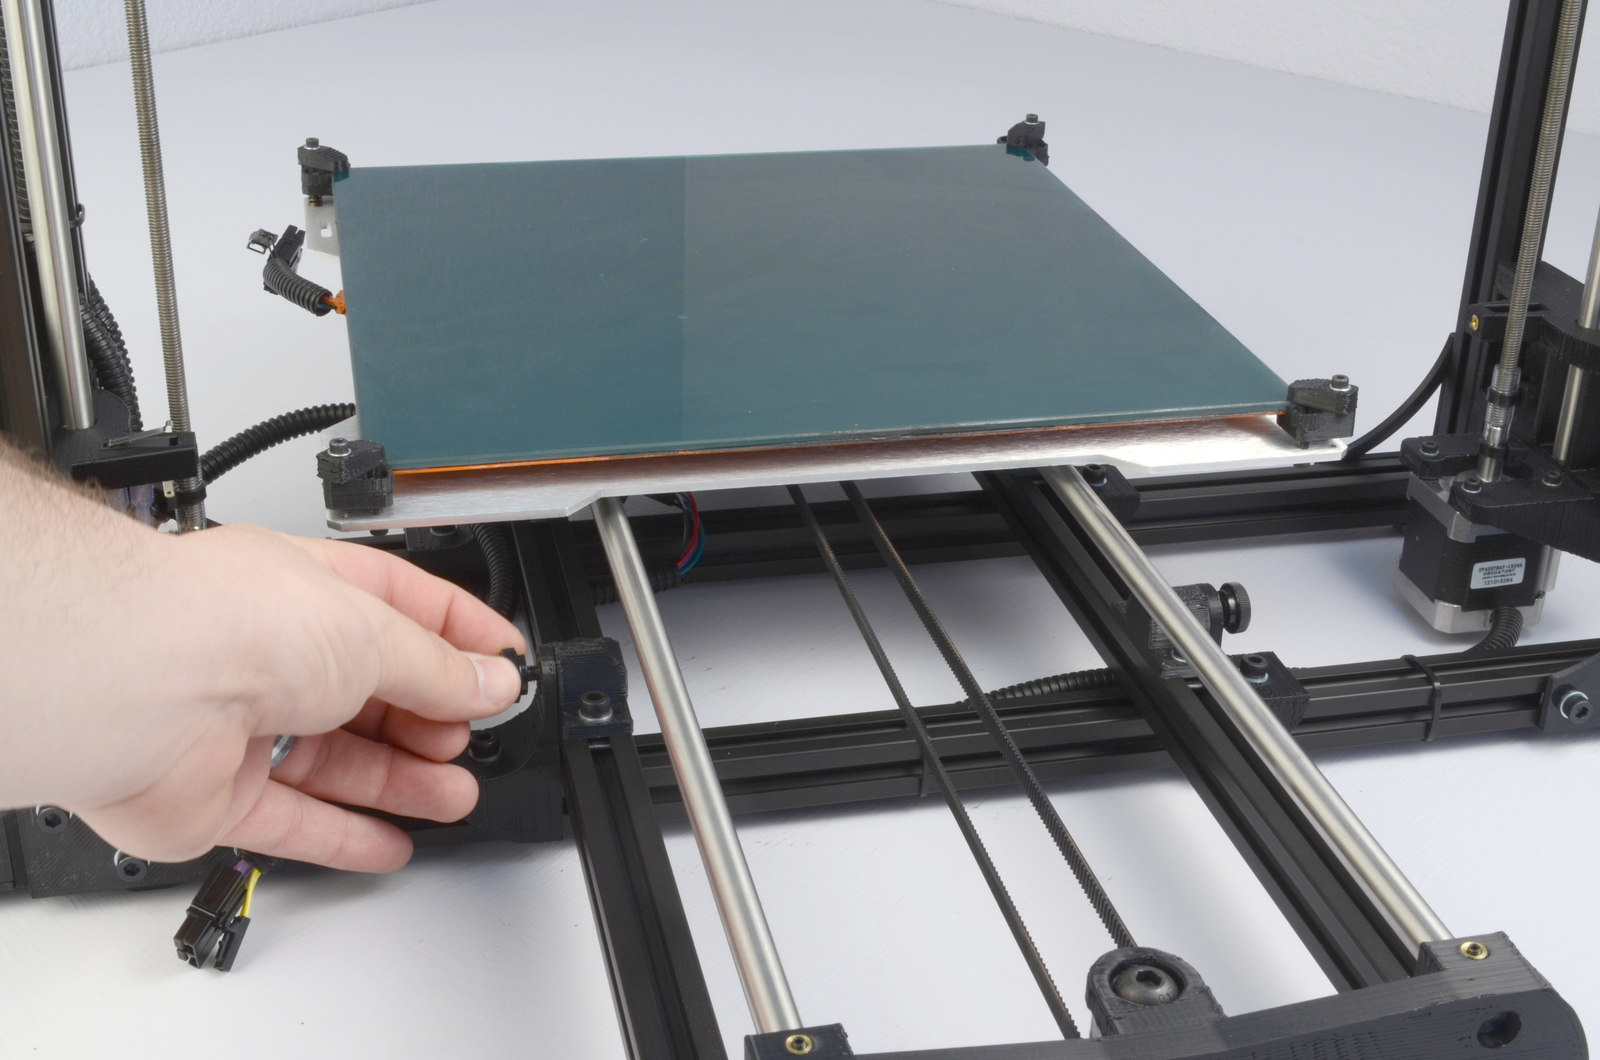
\includegraphics[keepaspectratio=true,angle=0,height=0.4\textheight,width=1.0\textwidth]{y_axis_bolt_tighten.JPG}
\caption{Screw in and tighten the four Y axis bolts}
\label{fig:Y_axis_bolts_tighten}
\end{figure}

\item The final step of installing the Y axis is connecting the print surface connectors and Y axis connectors. Pull the print bed completely to the front of the printer to get access to the Y axis connectors. You will find matching male and female 4 pin stepper motor connectors and two pin end stop connectors. Connect the matching male and female connectors (Fig. \ref{fig:Y_axis_connectors}, page \pageref{fig:Y_axis_connectors}); make sure the connector lock clicks to be sure that the connection is secure.


\begin{figure}[p]
\centering
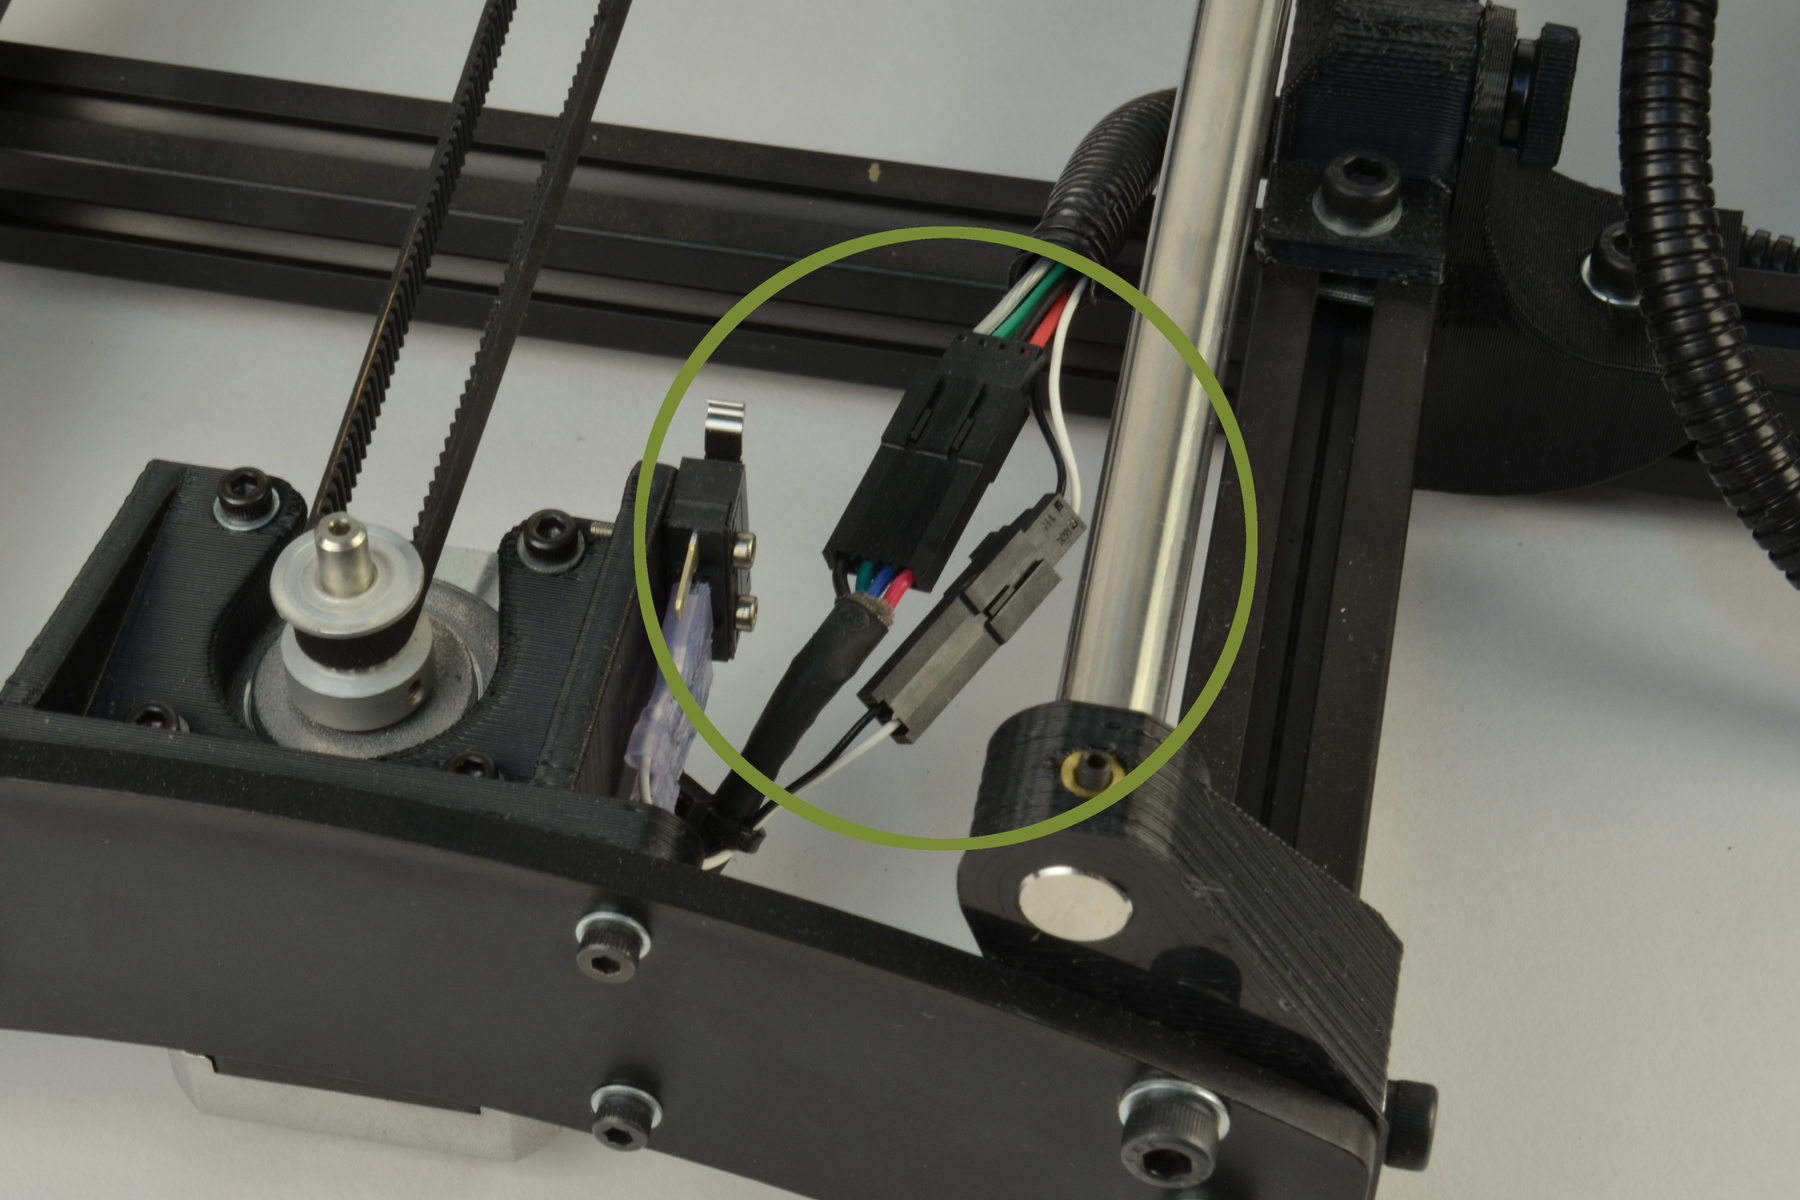
\includegraphics[keepaspectratio=true,angle=0,height=0.4\textheight,width=1.0\textwidth]{y_axis_connectors.JPG}
\caption{Connect the two connectors found at the rear of the Y axis}
\label{fig:Y_axis_connectors}
\end{figure}

\item Locate the two connectors to the left of the print bed. Connect the matching female and male large two pin heat bed connectors and the small two pin connectors (Fig. \ref{fig:bed_connectors}, page \pageref{fig:bed_connectors}).

\begin{figure}[p]
\centering
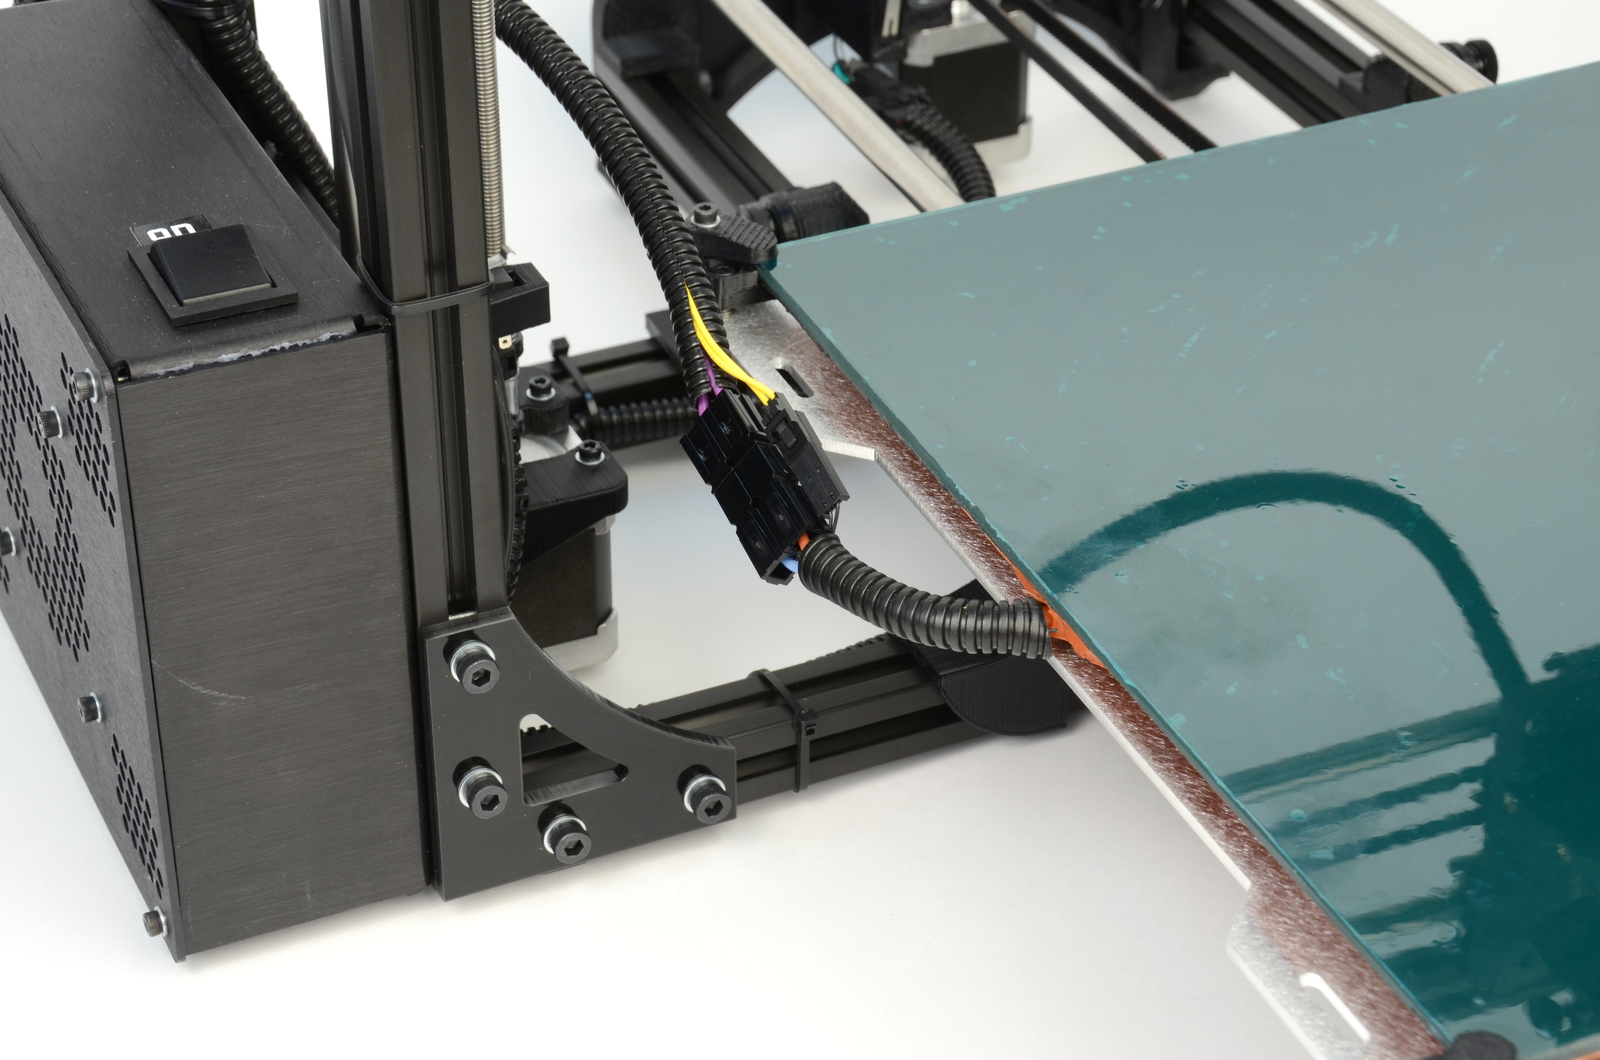
\includegraphics[keepaspectratio=true,angle=0,height=0.4\textheight,width=1.0\textwidth]{bed_connectors.JPG}
\caption{Connect the two connectors on the left of the print bed}
\label{fig:bed_connectors}
\end{figure}

\item Locate the two small black zip ties that are included in the documents bag (Fig. \ref{fig:bed_connectors_strain_relief}, page \pageref{fig:bed_connectors_strain_relief}). Wrap the two zip ties through the slot, located on the left rear of the aluminum bed plate, and around the print bed wires (Fig. \ref{fig:bed_connectors_strain_relief_done}, page \pageref{fig:bed_connectors_strain_relief_done}). Tighten the zip ties snug so the wire cannot move freely. Cut off the excess end of the zip ties with the needle nose pliers included in the tool bag.

%\begin{figure}[hp] CD forcing image placement
\begin{figure}[H]
\centering
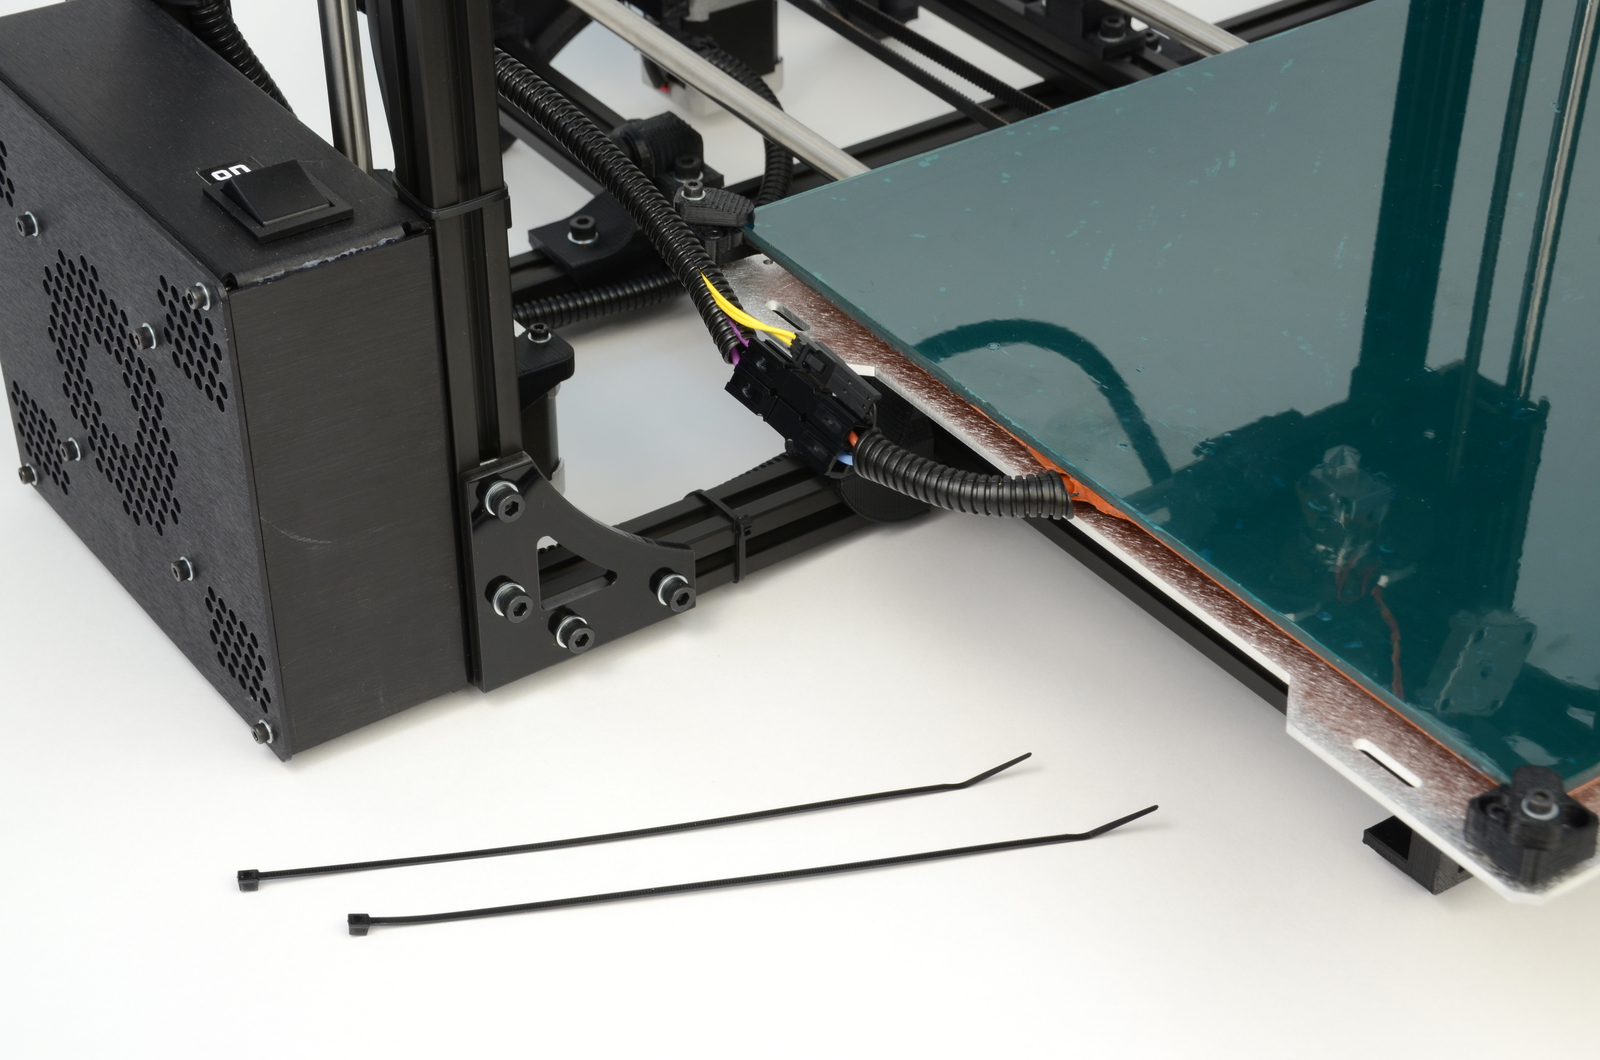
\includegraphics[keepaspectratio=true,angle=0,height=0.4\textheight,width=1.0\textwidth]{bed_connectors_strain_relief.JPG}
\caption{Locate the two zip ties found in the bag with the manual}
\label{fig:bed_connectors_strain_relief}
\end{figure}

%\begin{figure}[hp] CD forcing image placement
\begin{figure}[H]
\centering
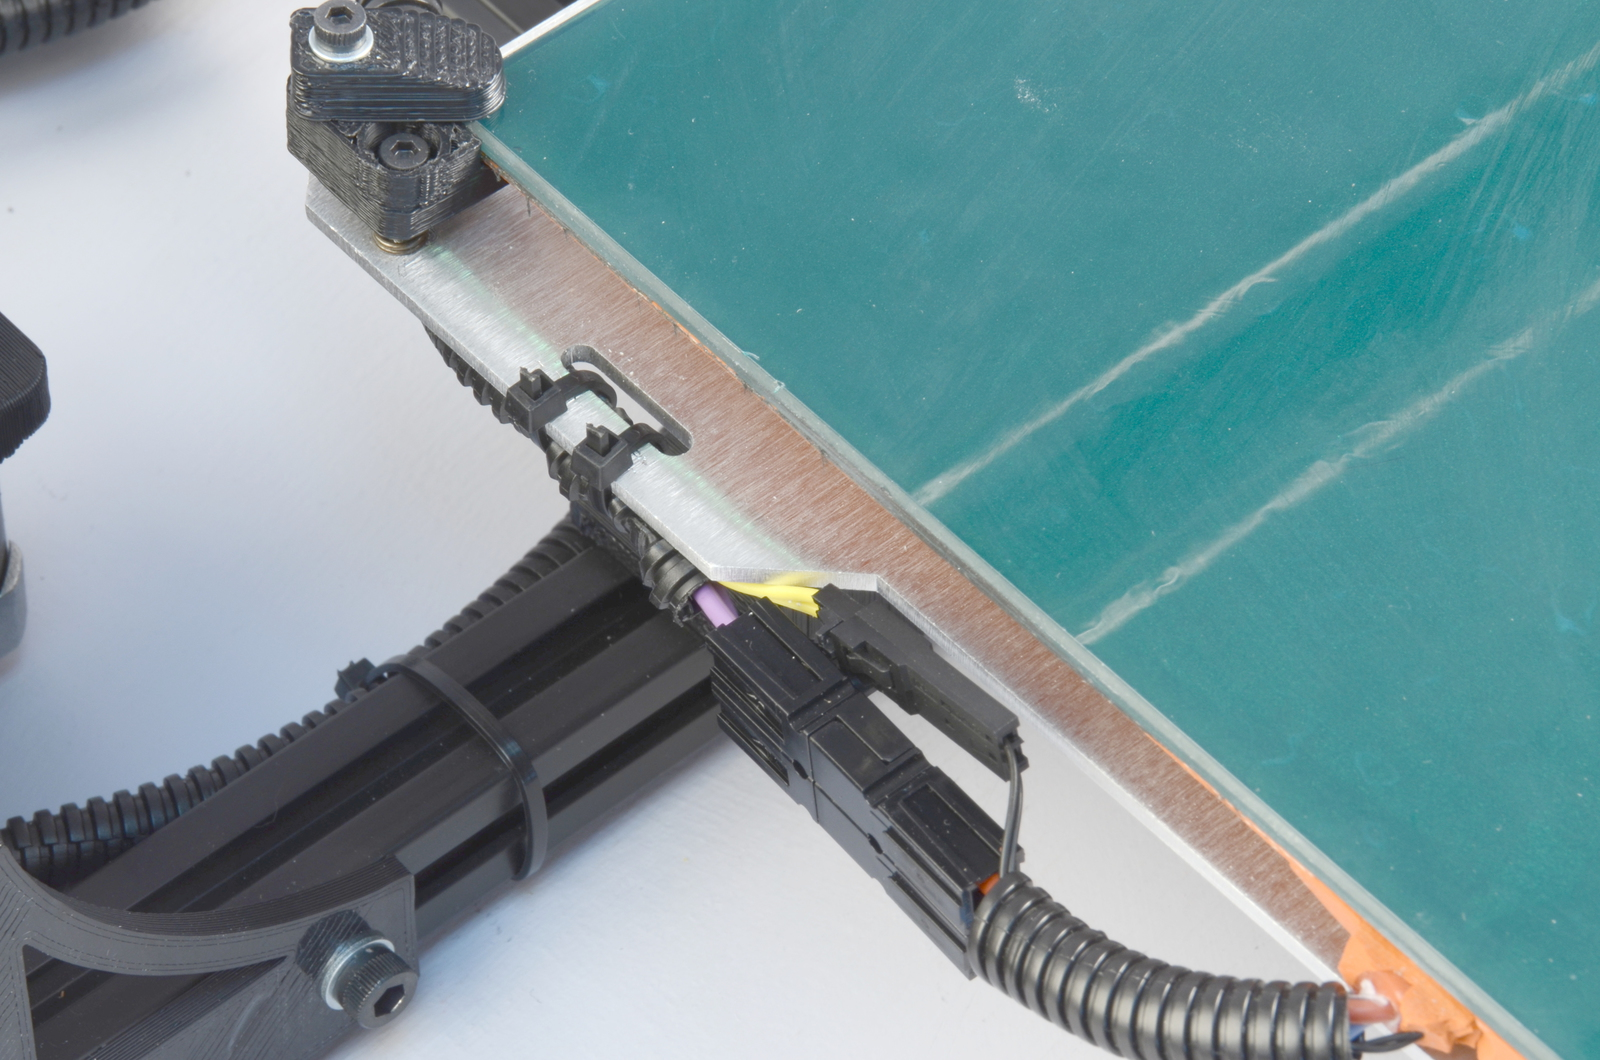
\includegraphics[keepaspectratio=true,angle=0,height=0.4\textheight,width=1.0\textwidth]{bed_connectors_strain_relief_done.JPG}
\caption{Tightly wrap the zip ties around the bed wires and through the strain relief slot}
\label{fig:bed_connectors_strain_relief_done}
\end{figure}

\item Move the X axis carriage to the center of the smooth rods. Remove the foam from between the X axis carriage and the left hand X axis end. Locate the extruder tool head screw from the accessories bag and place the extruder tool head onto the X axis carriage bottom first. The extruder mount will slide into the bottom portion of the carriage and self center. Use the included 2.5mm driver to secure the extruder tool head onto the X axis carriage.
\begin{figure}[hp]
\centering
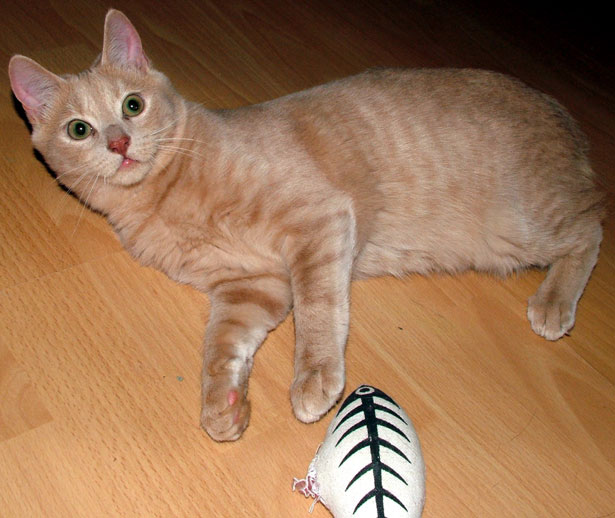
\includegraphics[keepaspectratio=true,angle=0,height=0.4\textheight,width=1.0\textwidth]{X_axis_toolhead.JPG}
\caption{Mount the extruder tool head}
\label{fig:X_axis_toolhead}
\end{figure}

\item Connect the stepper motor and the hot end to the existing wiring harness.  You will find matching male and female 4 pin stepper motor connectors and two pin end stop connectors. Connect the matching male and female connectors (Fig. \ref{fig:X_axis_connectors}, page \pageref{fig:X_axis_connectors}); make sure the connector lock clicks to be sure that the connections are secure.
\begin{figure}[hp]
\centering
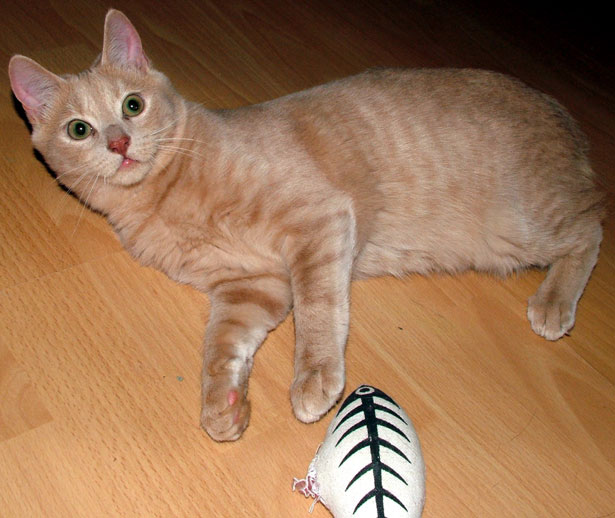
\includegraphics[keepaspectratio=true,angle=0,height=0.4\textheight,width=1.0\textwidth]{X_axis_connectors.JPG}
\caption{Extruder connections}
\label{fig:X_axis_connectors}
\end{figure}

\item Secure the wiring harness into the strain relief on the top left hand side of the X axis carriage. 
\begin{figure}[hp]
\centering
\includegraphics[keepaspectratio=true,angle=0,height=0.4\textheight,width=1.0\textwidth]{X+axis_strain_relief.JPG}
\caption{Strain relief installation}
\label{fig:X_axis_strain_relief}
\end{figure}

\item Now that the Y axis is mounted and the extruder tool head is installed you should set your printer on a stable, flat, and level surface large enough for extra space around the printer. Make sure your printer work space is clear of anything that could obstruct the movement of the printer. Move the Y axis to the back of the printer to ensure unobstructed movement of that axis. \textcolor{red}{Make sure there are no flammable fabrics or liquids near the printer space}. It is also best to not put your printer near a drafty window or air conditioner vent.

\index{power supply}
\index{USB cable}
\item Unwrap the power supply and USB cables.

\textcolor{red}{MAKE SURE THE POWER SUPPLY IS COMPLETELY UNPLUGGED BEFORE MOVING ON TO THE NEXT STEP}.

\index{electronics receptacles}
\item Locate the power supply and USB receptacles along the back of the TAZ electronics enclosure
(Fig. \ref{fig:electronics_plugs}, page \pageref{fig:electronics_plugs}). Locate the power supply and the included AC power cable (Fig. \ref{fig:power_supply}, page \pageref{fig:power_supply}). Locate the DC power cable plug on the power supply. Connect the DC locking plug into the DC connector on the TAZ electronics enclosure (Fig. \ref{fig:ps_plug}, page \pageref{fig:ps_plug}). The plug is keyed which may require rotating the plug until the keys line up and the plug can be pushed in. Once you have pushed in the plug turn the locking sleeve clockwise until it is tight against the electronics enclosure (Fig. \ref{fig:electronics_plugs_plugged-in}, page \pageref{fig:electronics_plugs_plugged-in}).
%\begin{figure}[hbt]
\begin{figure}[H]
\centering
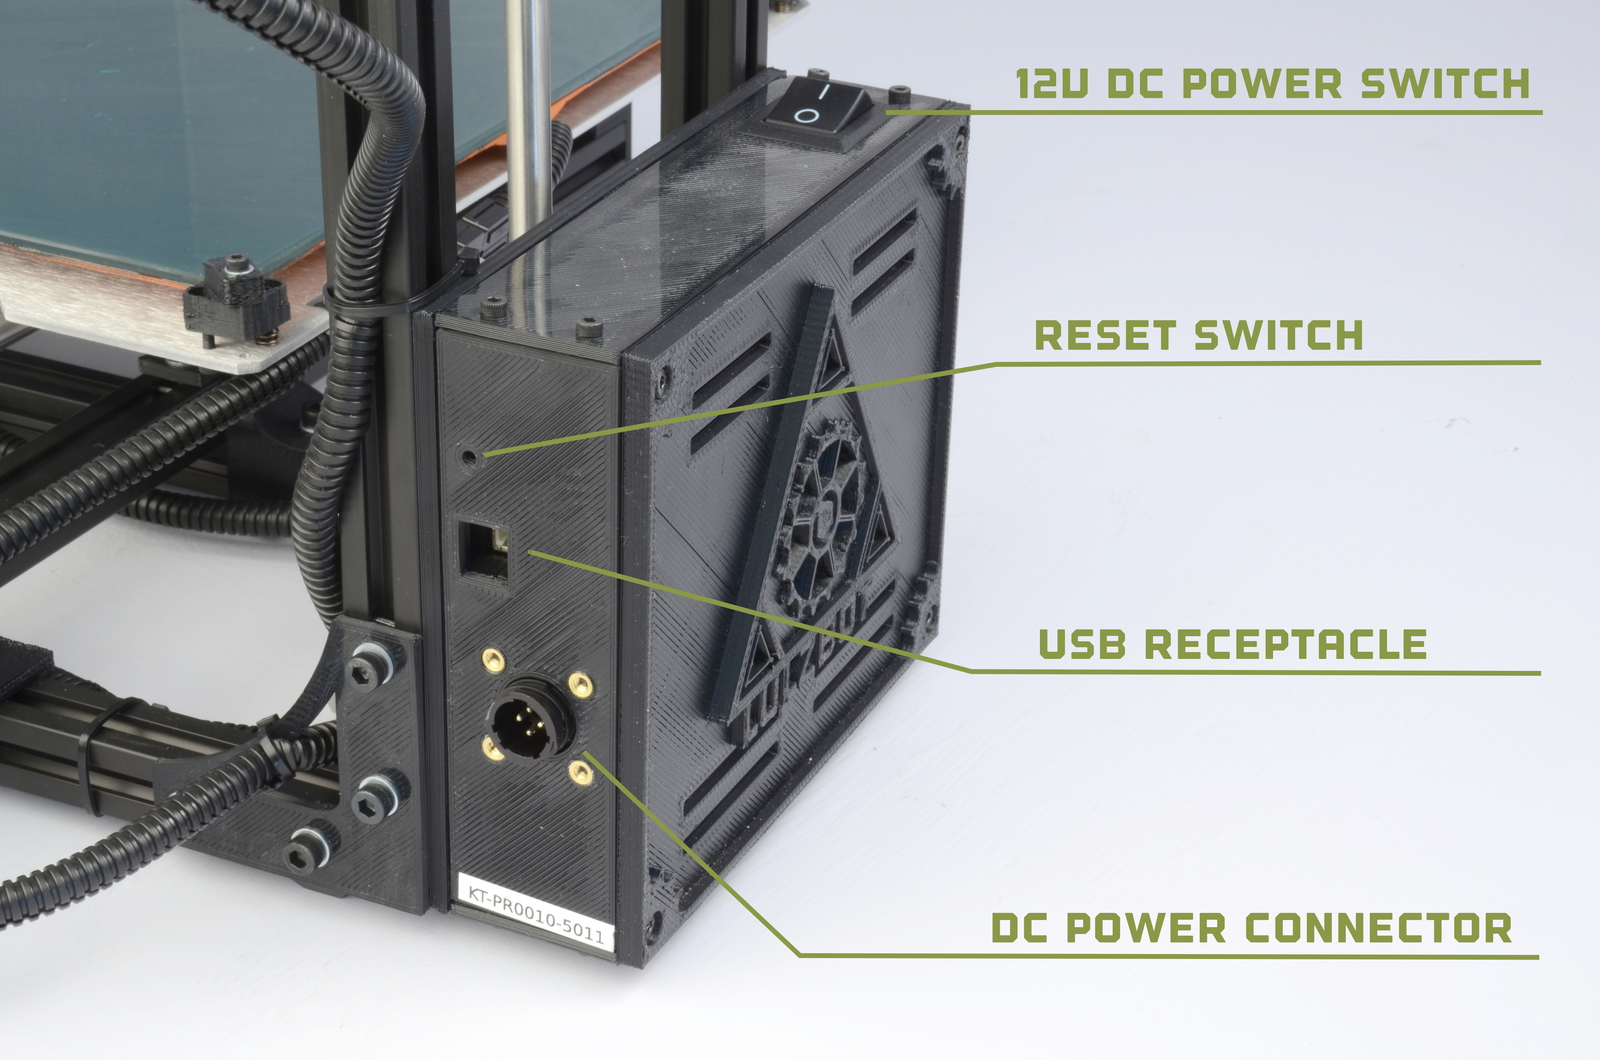
\includegraphics[keepaspectratio=true,angle=0,height=0.4\textheight,width=1.0\textwidth]{electronics_case_rec.JPG}
\caption{Power supply and USB receptacles}
\label{fig:electronics_plugs}
\end{figure}

%\begin{figure}[hp]
\begin{figure}[H]
\centering
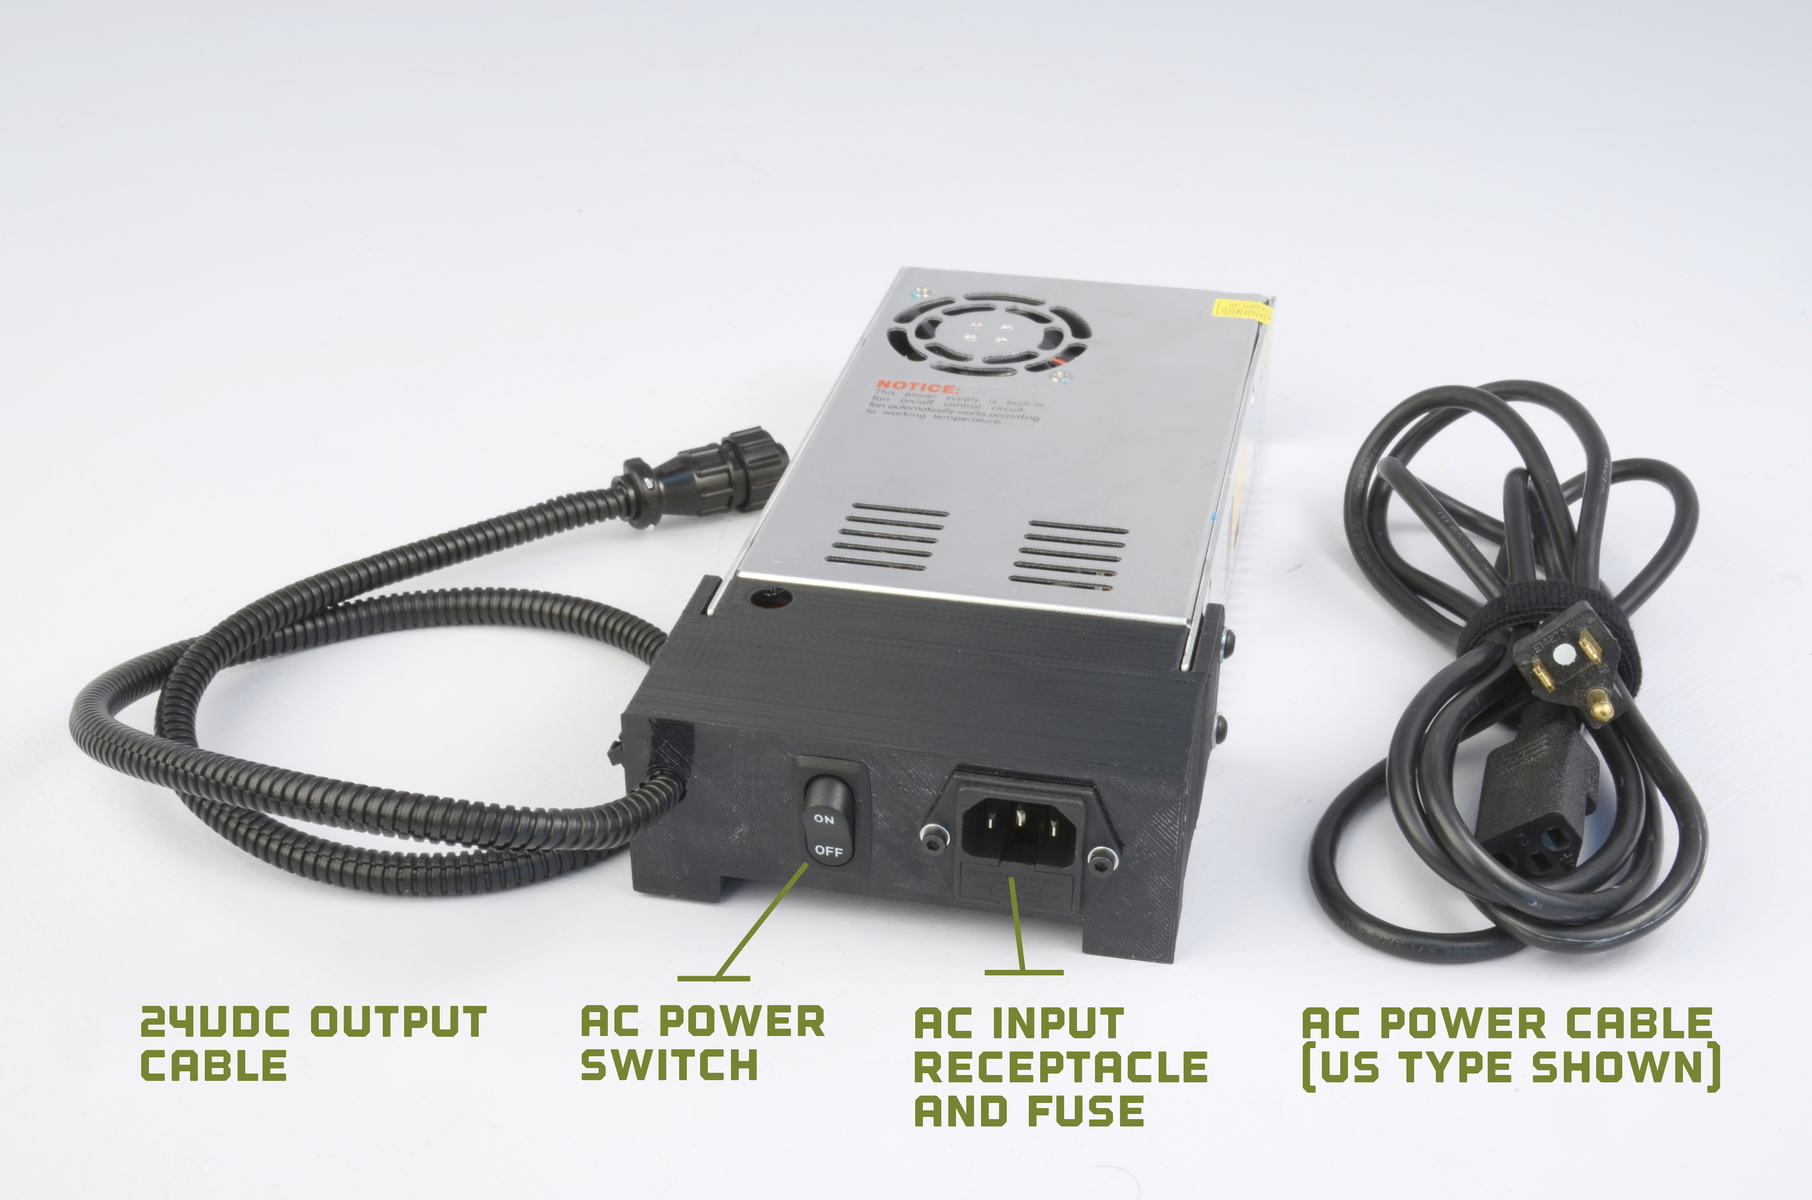
\includegraphics[keepaspectratio=true,angle=0,height=0.4\textheight,width=1.0\textwidth]{power_supply.JPG}
\caption{Power supply}
\label{fig:power_supply}
\end{figure}

%\begin{figure}[hp]
\begin{figure}[H]
\centering
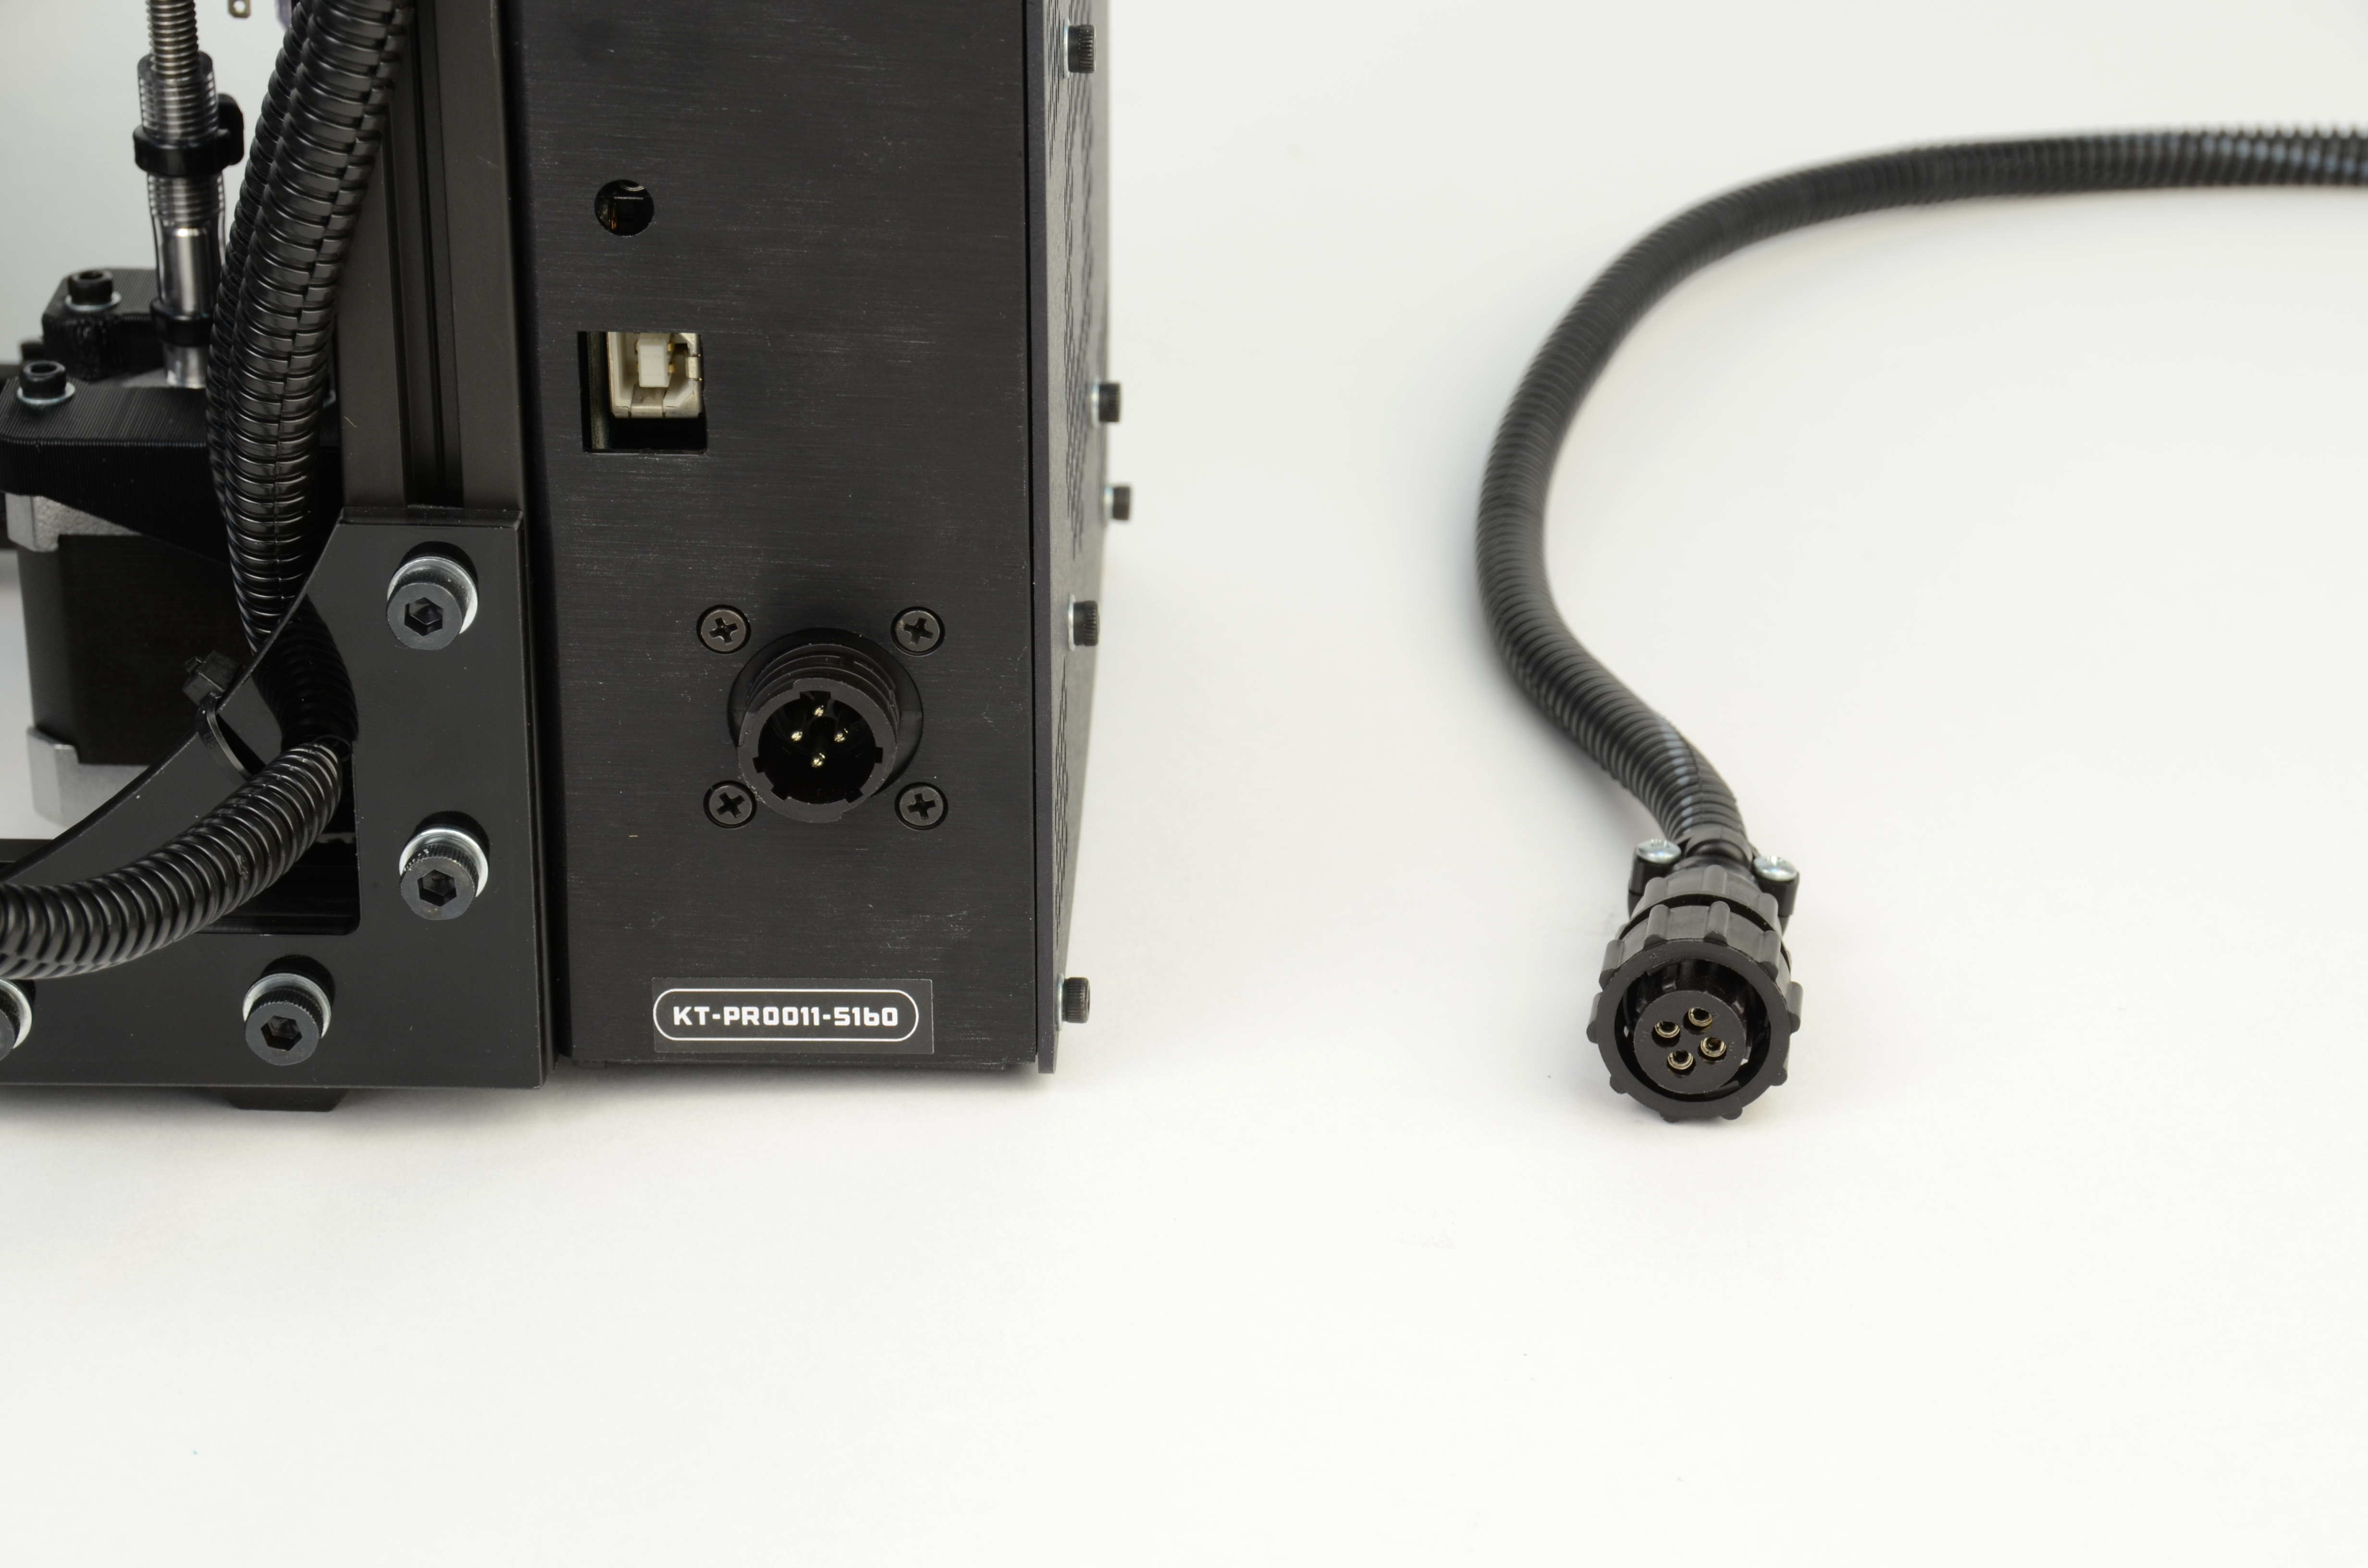
\includegraphics[keepaspectratio=true,angle=0,height=0.4\textheight,width=1.0\textwidth]{electronics_DC_connector.JPG}
\caption{12V DC Power supply plug and receptacle}
\label{fig:ps_plug}
\end{figure}

%\begin{figure}[hp]
\begin{figure}[H]
\centering
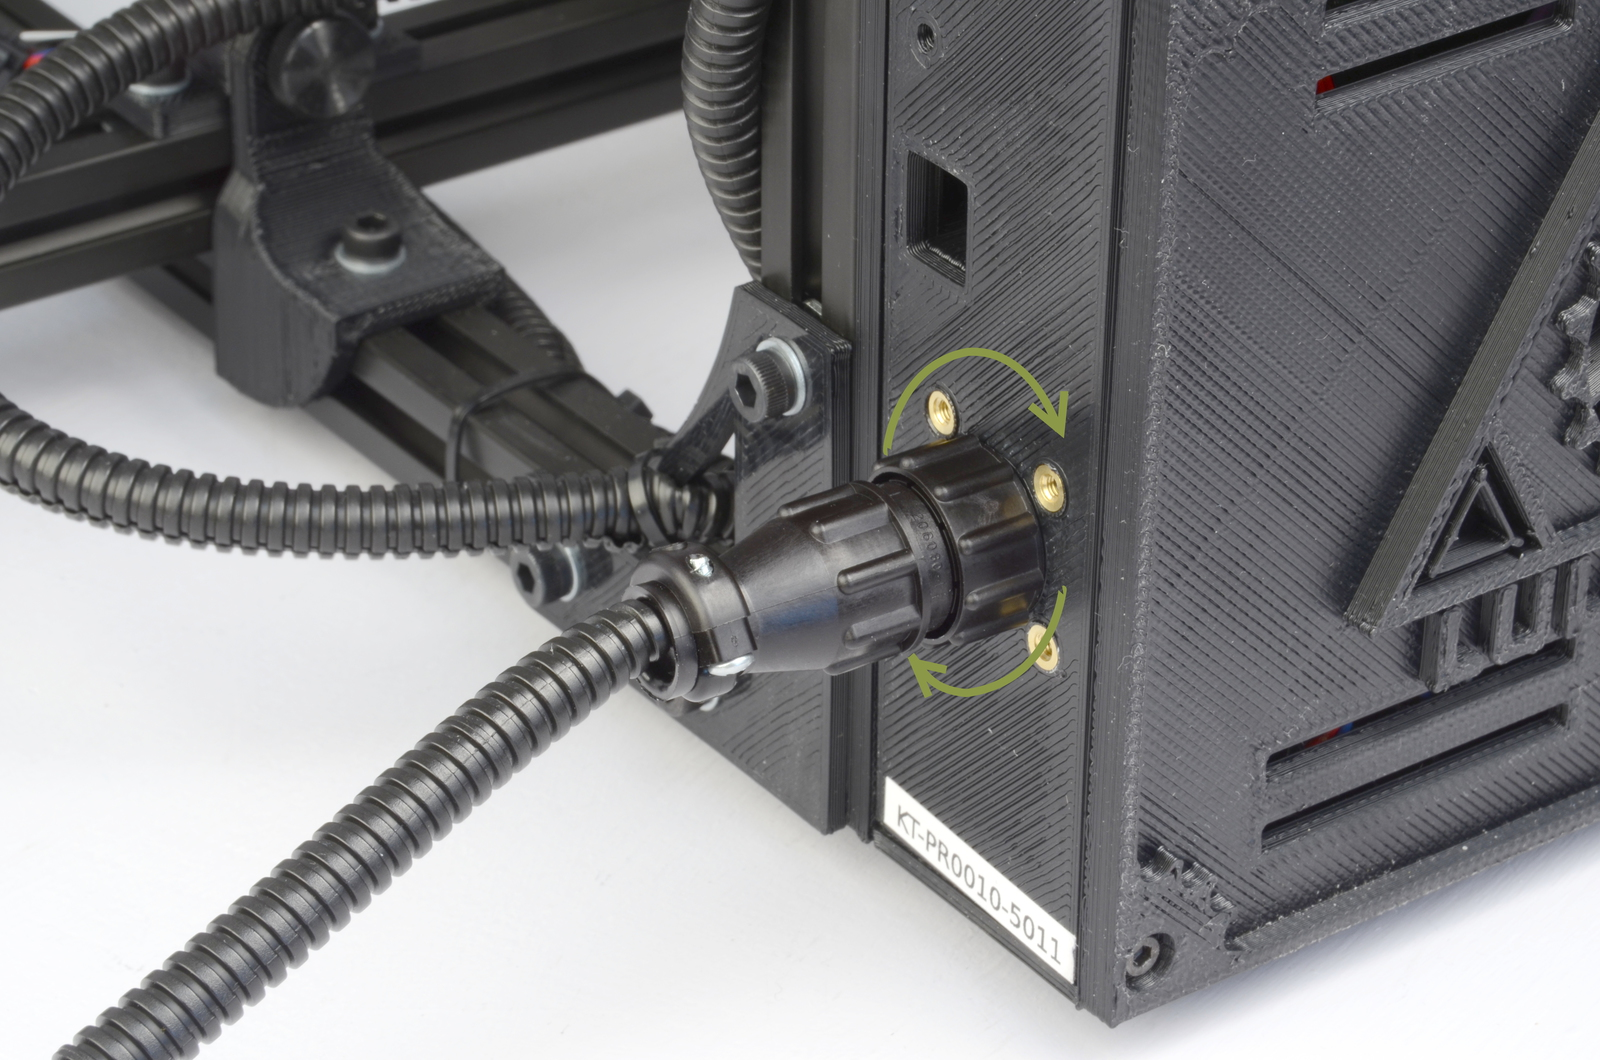
\includegraphics[keepaspectratio=true,angle=0,height=0.4\textheight,width=1.0\textwidth]{electronics_DC_connector_tight.JPG}
\caption{The power supply plug correctly plugged in}
\label{fig:electronics_plugs_plugged-in}
\end{figure}

\item Locate, on the right of the power supply, the red AC voltage switch. Depending on your location you will need to change the AC voltage switch to 115V or 230V. North America is generally 115V and the majority of other regions are 230V. You can find general voltage by country at \texttt{wikipedia.org/wiki/Mains\_electricity\_by\_country}. Make sure that when plugging in the AC power cable it is directly plugged into the wall and \textbf{not} into a power strip. The TAZ 3D printer can potentially pull more current than the power strip will support and may lead to undesirable performance. 

\index{RAMBo}
\item Plug in the USB cable, B plug (square plug) side, into the USB receptacle on the printer electronics. Plug the other end of the USB cable, A plug side, into your computer.

\index{PTFE tube}
\item Locate the filament guide with attached PTFE tube
(Fig. \ref{fig:filament_guide}, page \pageref{fig:filament_guide}). The filament guide attaches to the filament guide mount which can be found on the top right side of the printer frame (Fig. \ref{fig:filament_guide_mount}, page \pageref{fig:filament_guide_mount}). The filament guide easily pops on to the guide mount as shown in figure \ref{fig:filament_guide_setting} (pg. \pageref{fig:filament_guide_setting}).
%\begin{figure}[hbt]
\begin{figure}[H]
\centering
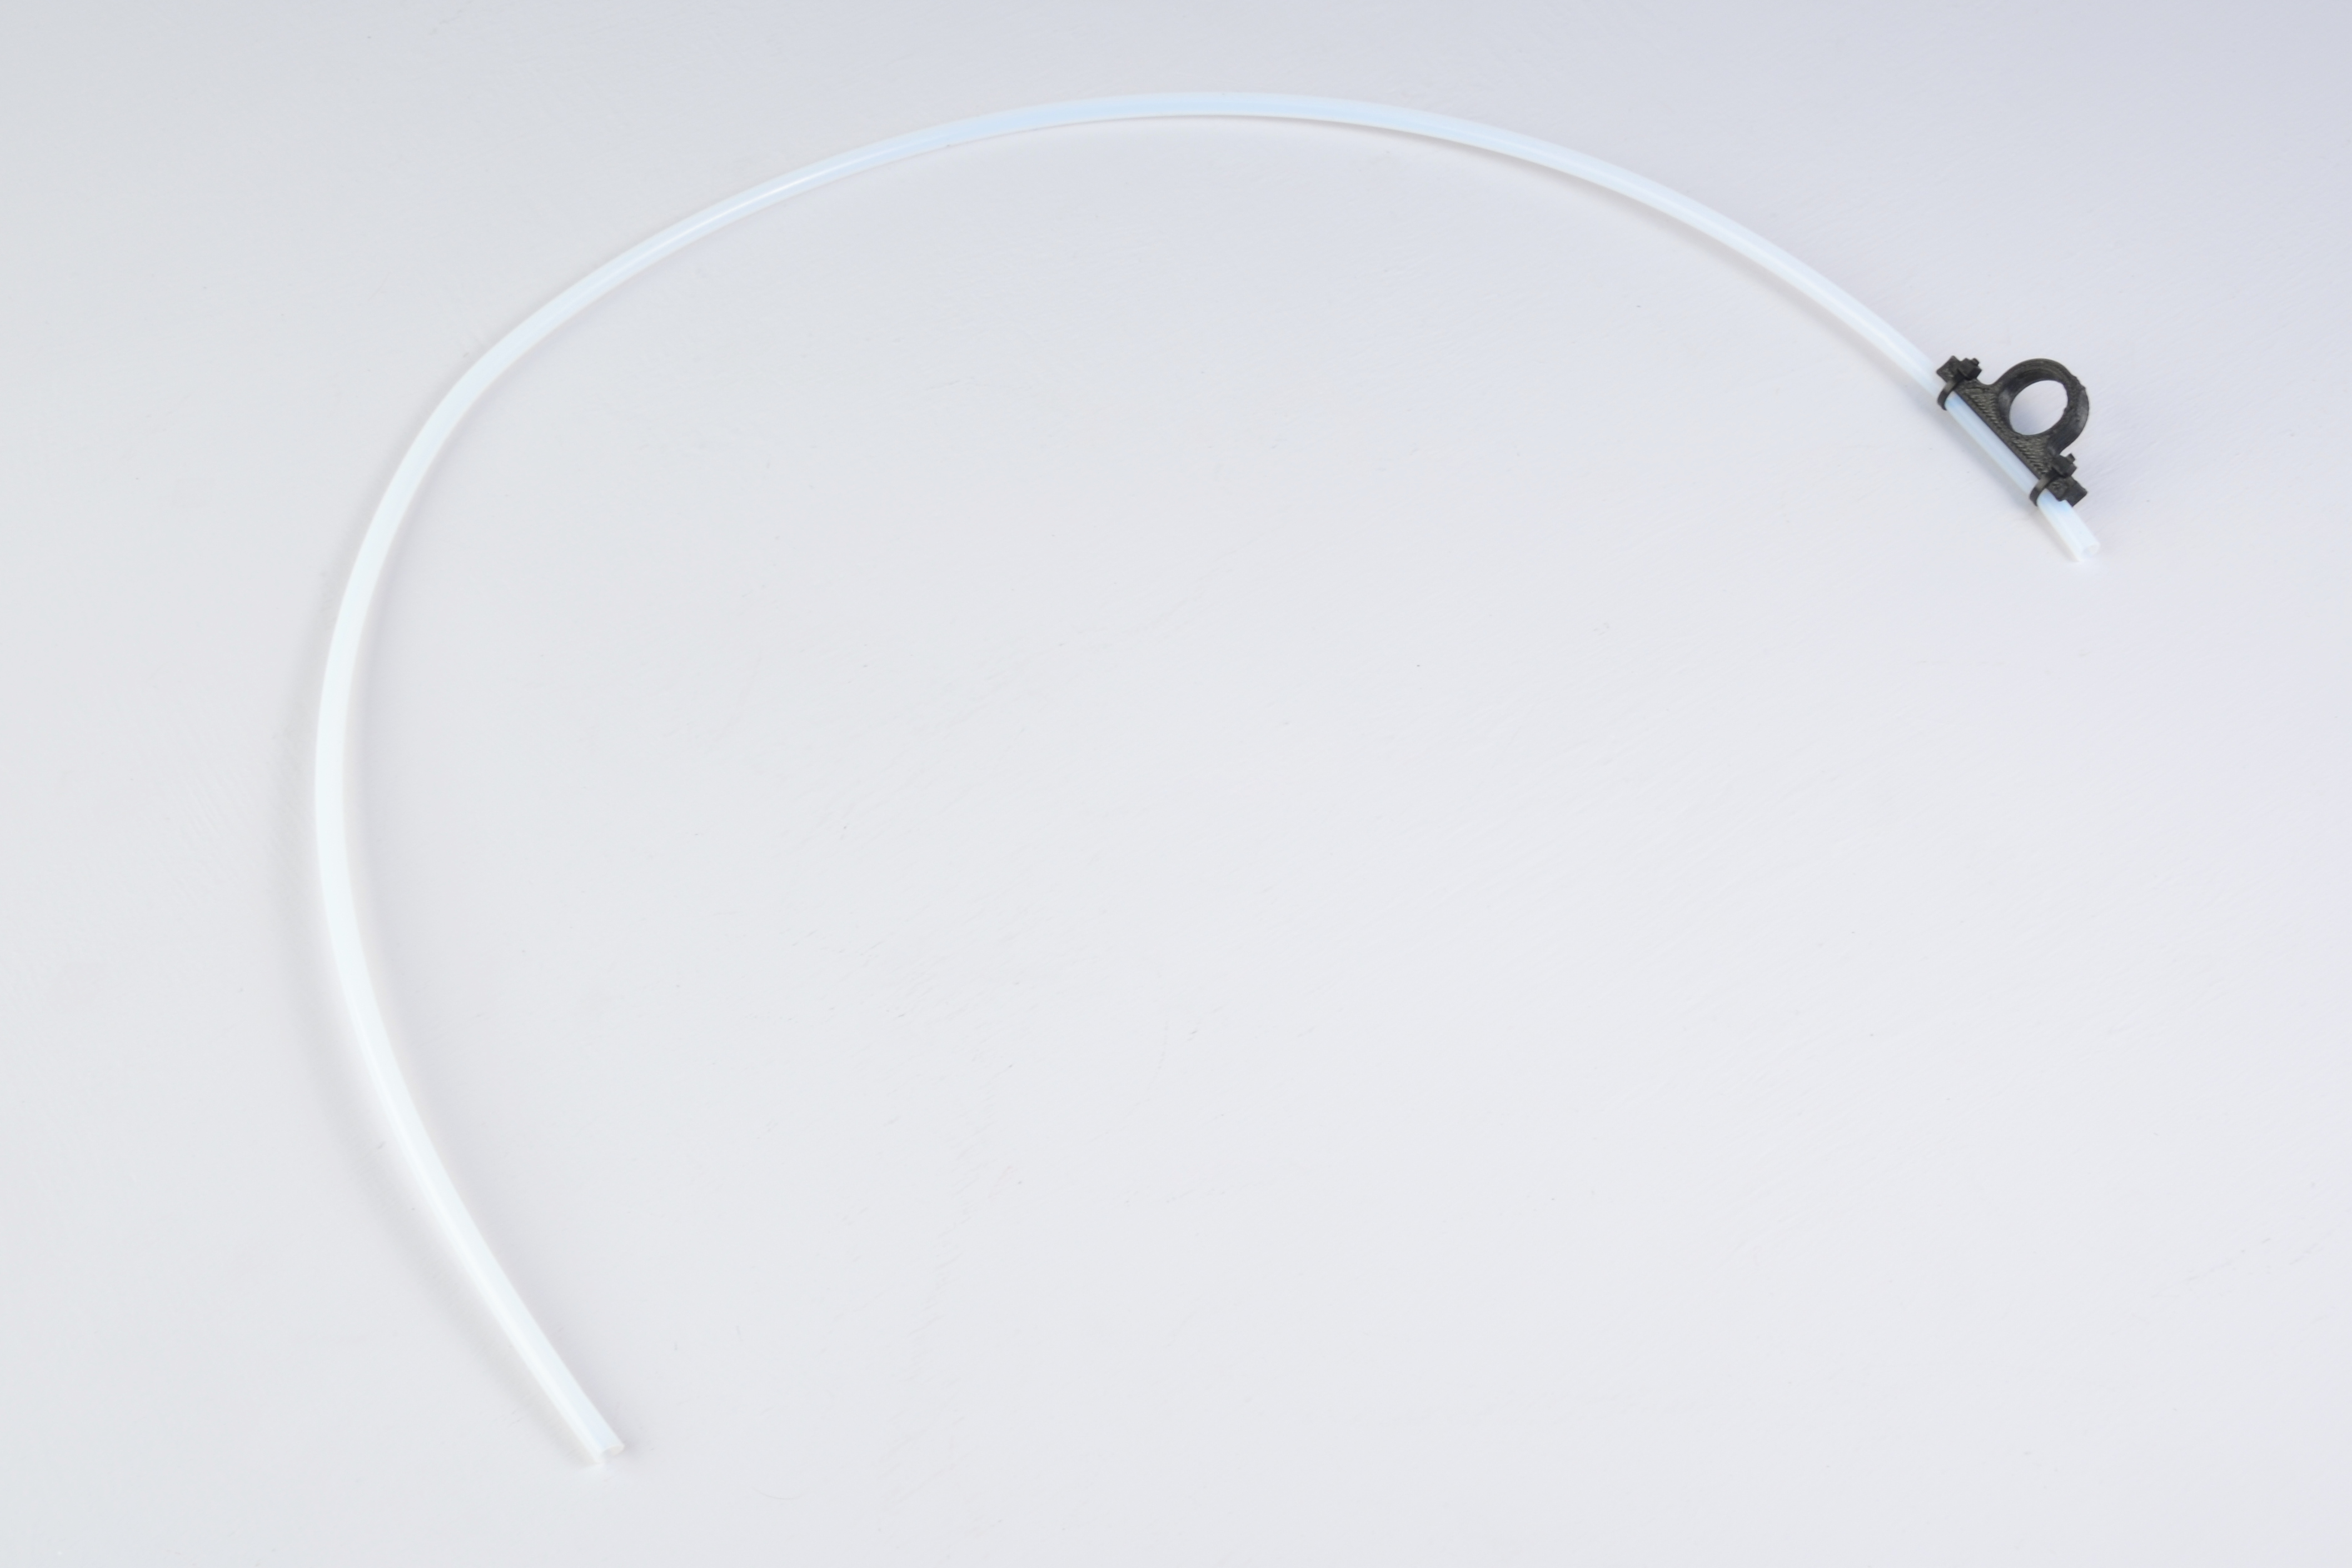
\includegraphics[keepaspectratio=true,angle=0,height=0.4\textheight,width=1.0\textwidth]{filament_guide.JPG}
\caption{Filament Guide}
\label{fig:filament_guide}
\end{figure}

%\begin{figure}[hbt]
\begin{figure}[H]
\centering
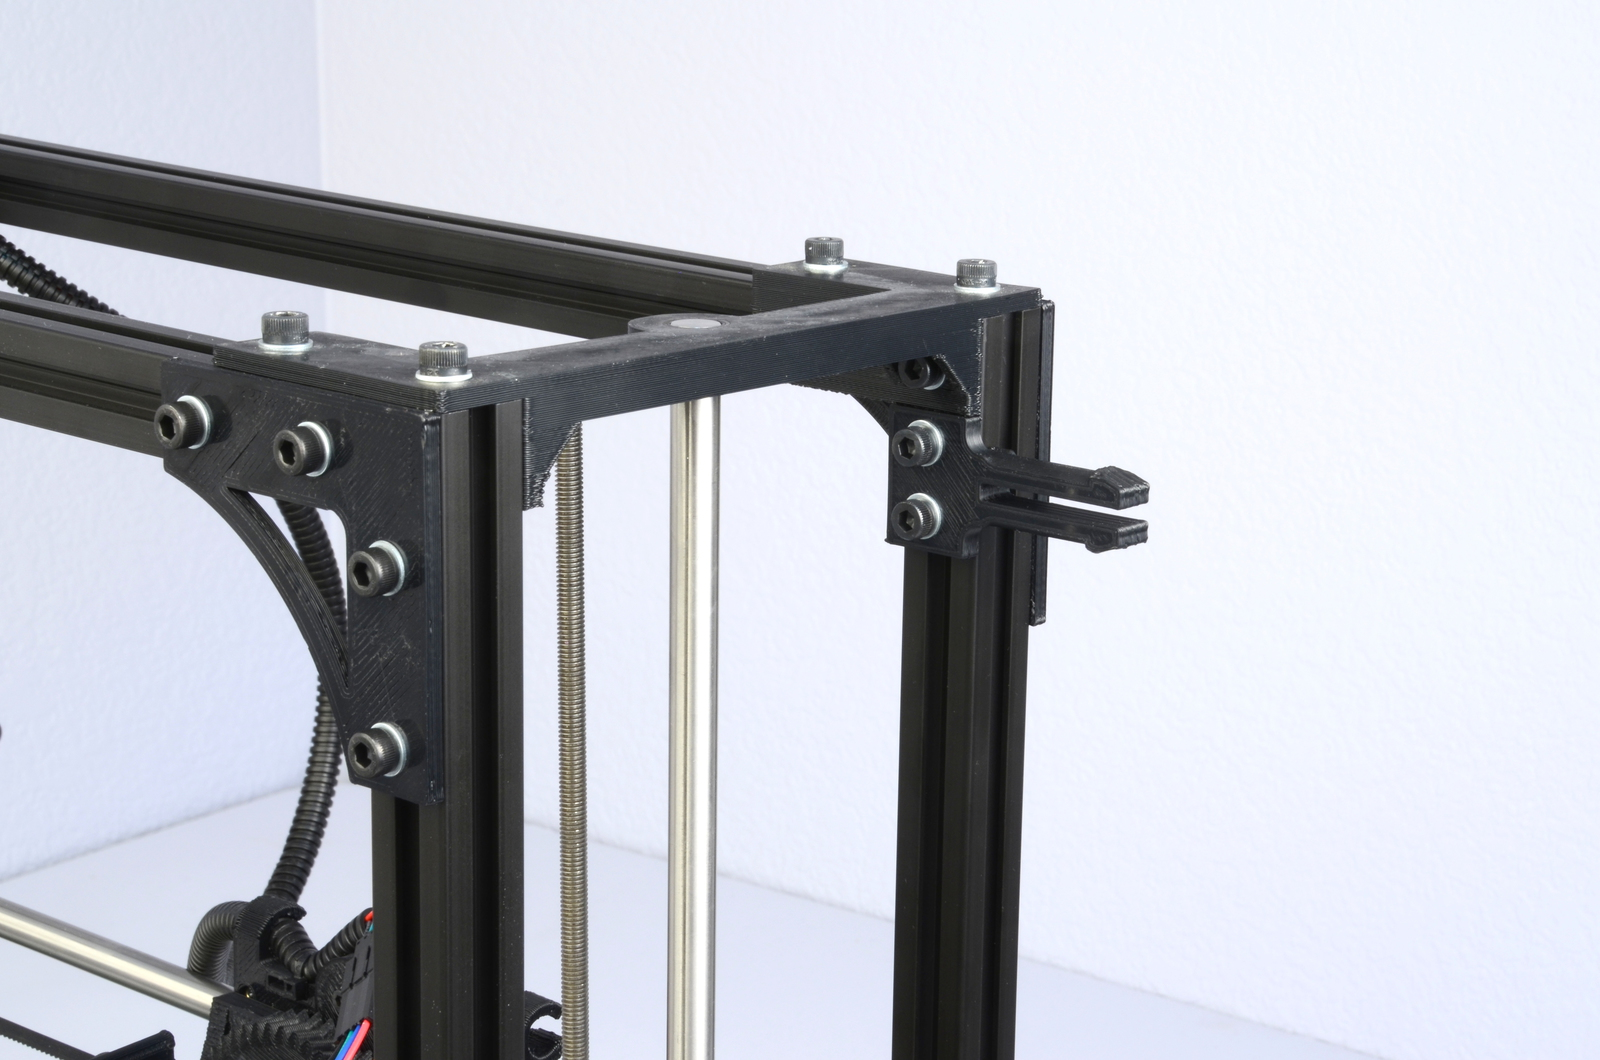
\includegraphics[keepaspectratio=true,angle=0,height=0.4\textheight,width=1.0\textwidth]{filament_guide_mount.JPG}
\caption{Filament Guide Mount}
\label{fig:filament_guide_mount}
\end{figure}

%\begin{figure}[hbt]
\begin{figure}[H]
\centering
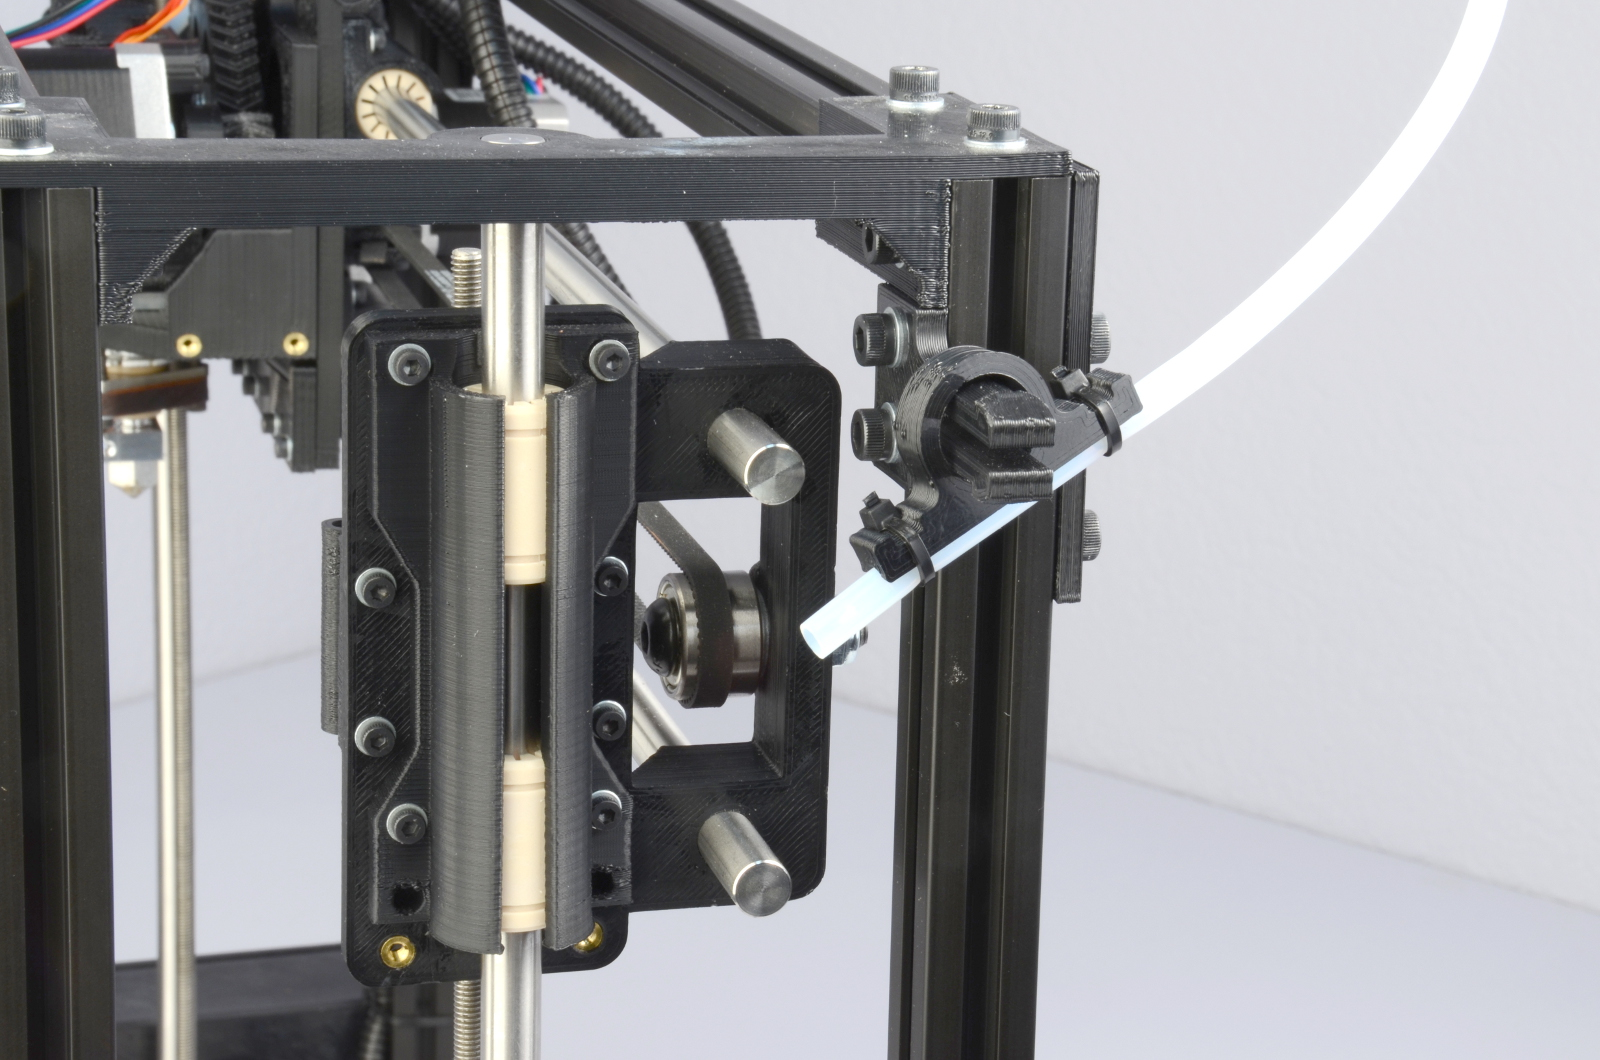
\includegraphics[keepaspectratio=true,angle=0,height=0.4\textheight,width=1.0\textwidth]{filament_guide_direction.JPG}
\caption{Filament Guide Setting}
\label{fig:filament_guide_setting}
\end{figure}

\index{end stops}
\glossary{End stops}{Mechanical or optical switches that are used to mark the 3 home (zero) positions.}
\item Your TAZ 3D printer is now setup and ready to start printing. Before moving forward you should become familiar with the TAZ Cartesian type system. The printer moves in three axes: X, Y, and Z (Fig. \ref{fig:axes}, page \pageref{fig:axes}). These three axes allow the tool head to move to any point within the print area. Note the location of the mechanical end stops which are small switches located at the home point of each axis (Fig. \ref{fig:endstops}, page \pageref{fig:endstops}). Each end stop switch allows the printer to find the 0, the origin, or starting point, of each axis. The mechanical end stops should never be blocked during the initial homing function or during a print.
%\begin{figure}[hbt]
\begin{figure}[H]
\centering
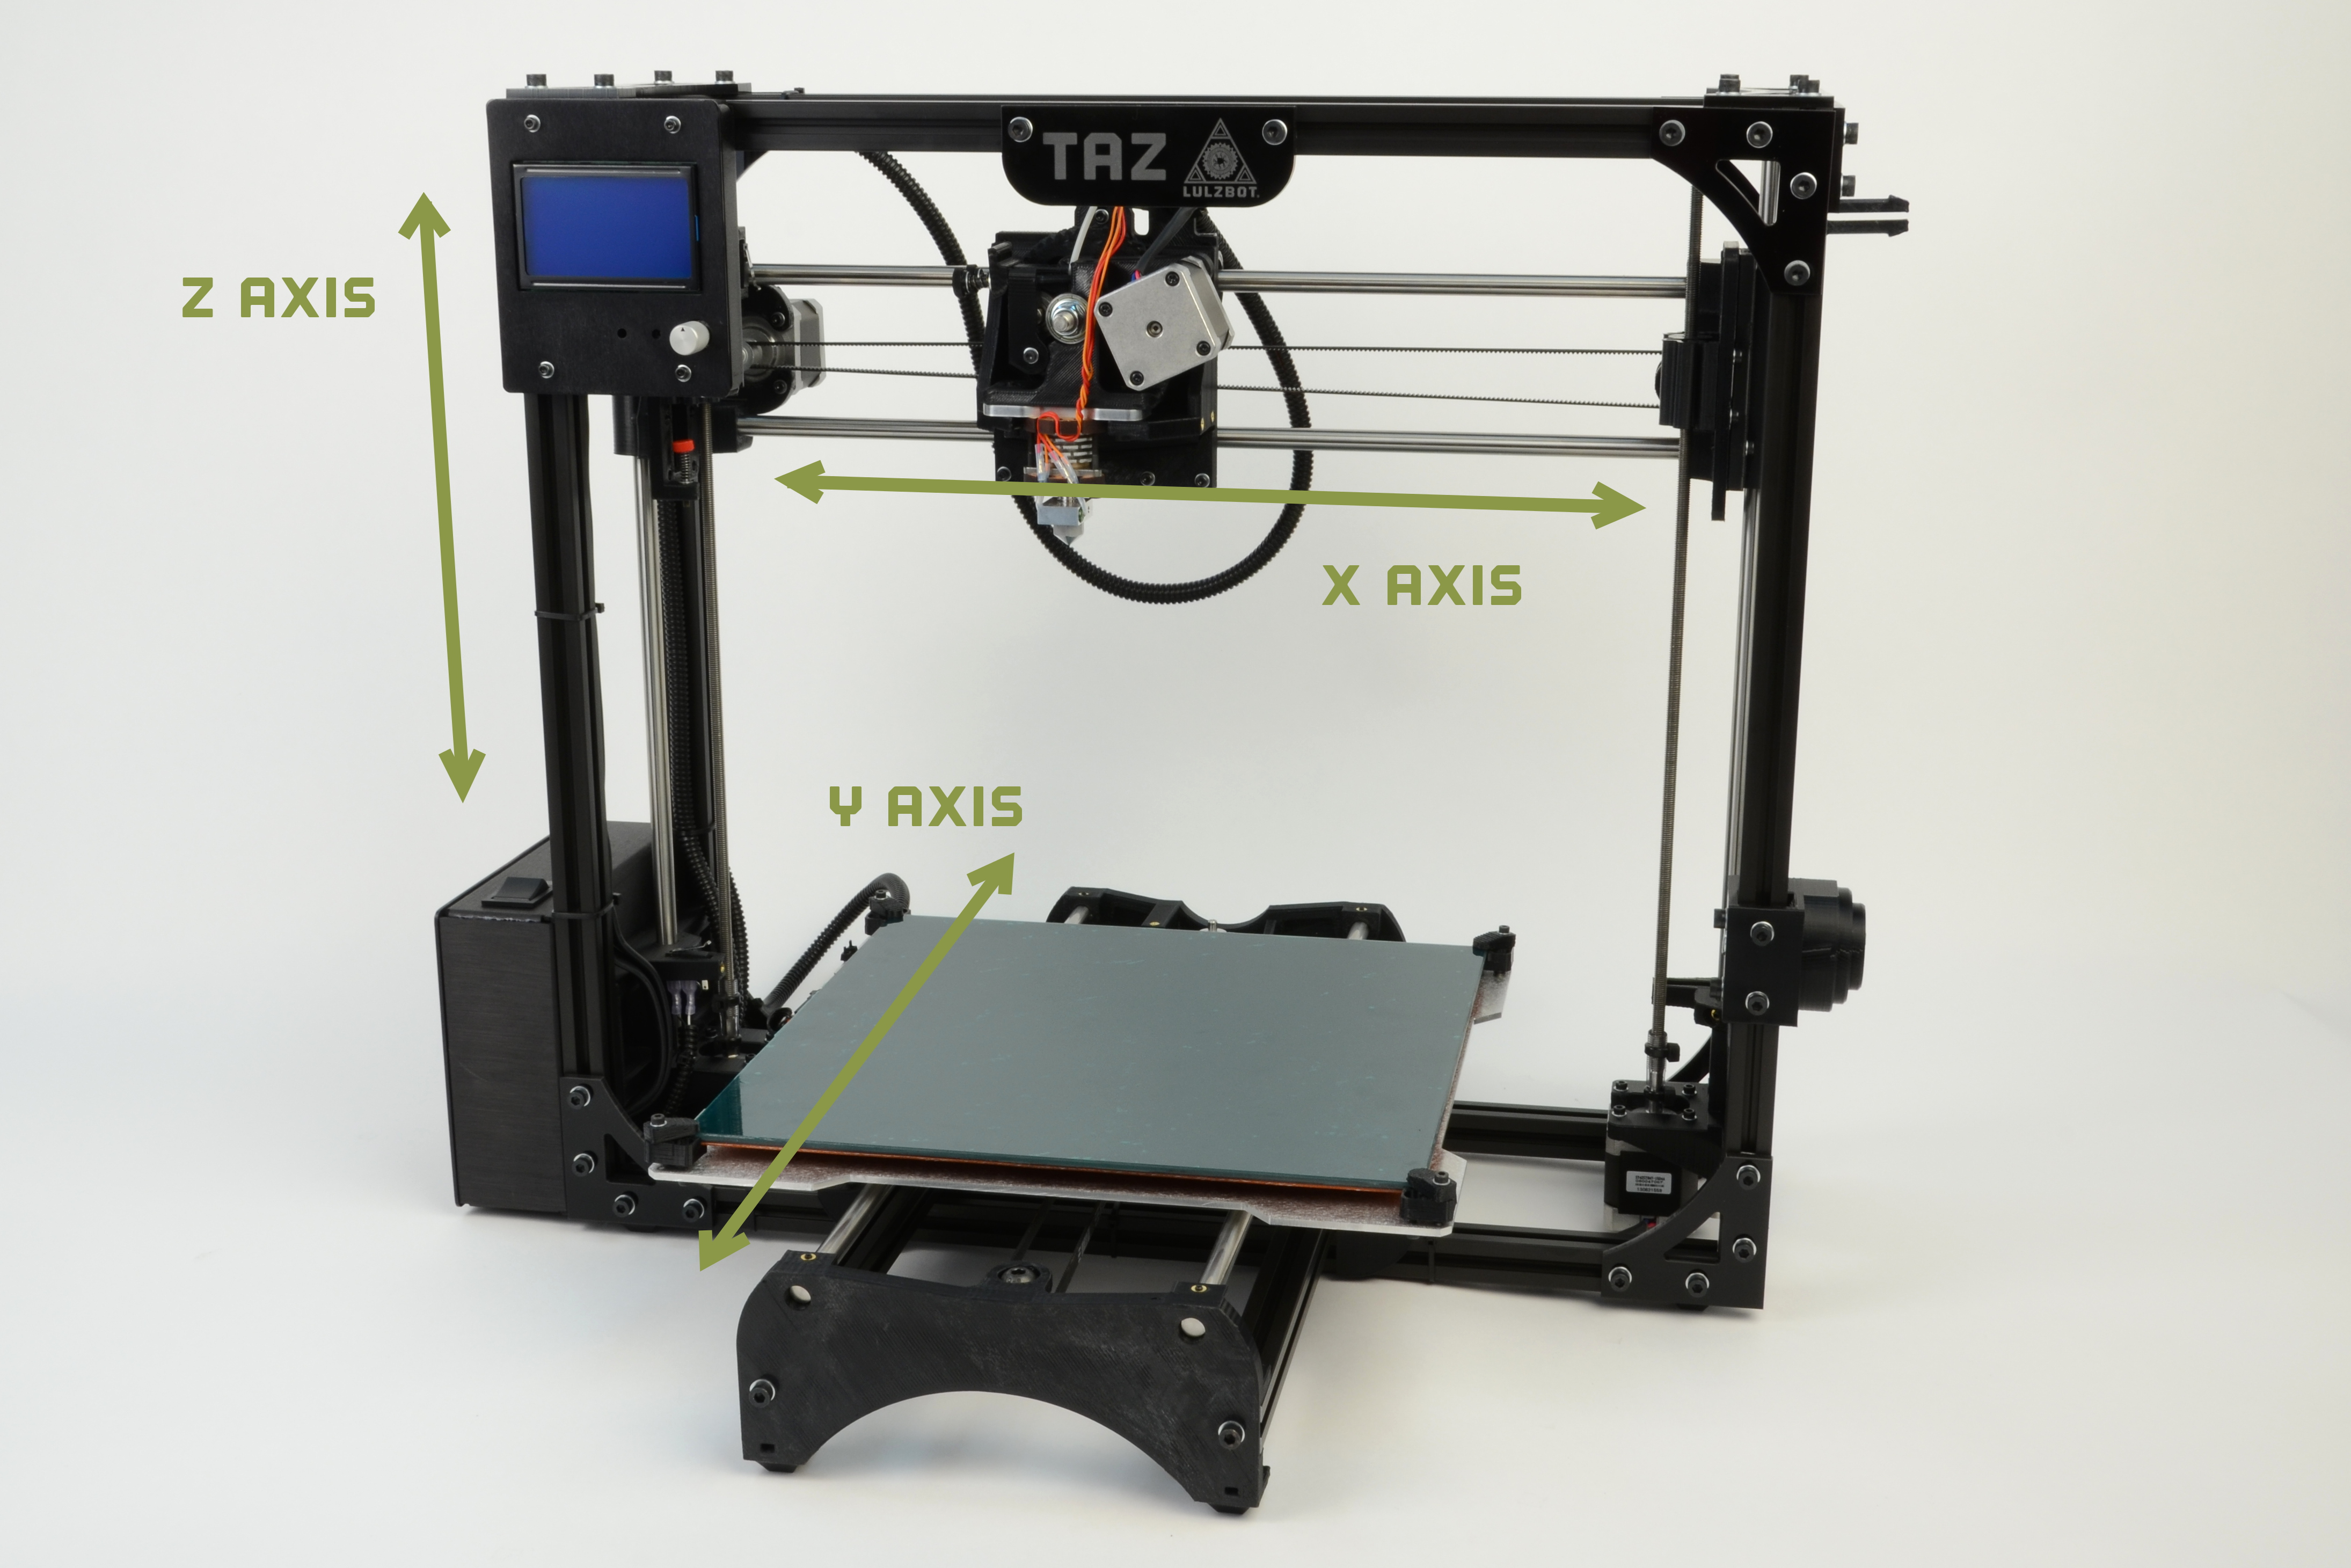
\includegraphics[keepaspectratio=true,angle=0,height=0.4\textheight,width=1.0\textwidth]{axes.JPG}
\caption{Axes movement directions}
\label{fig:axes}
\end{figure}

\begin{figure}[hp]
\centering
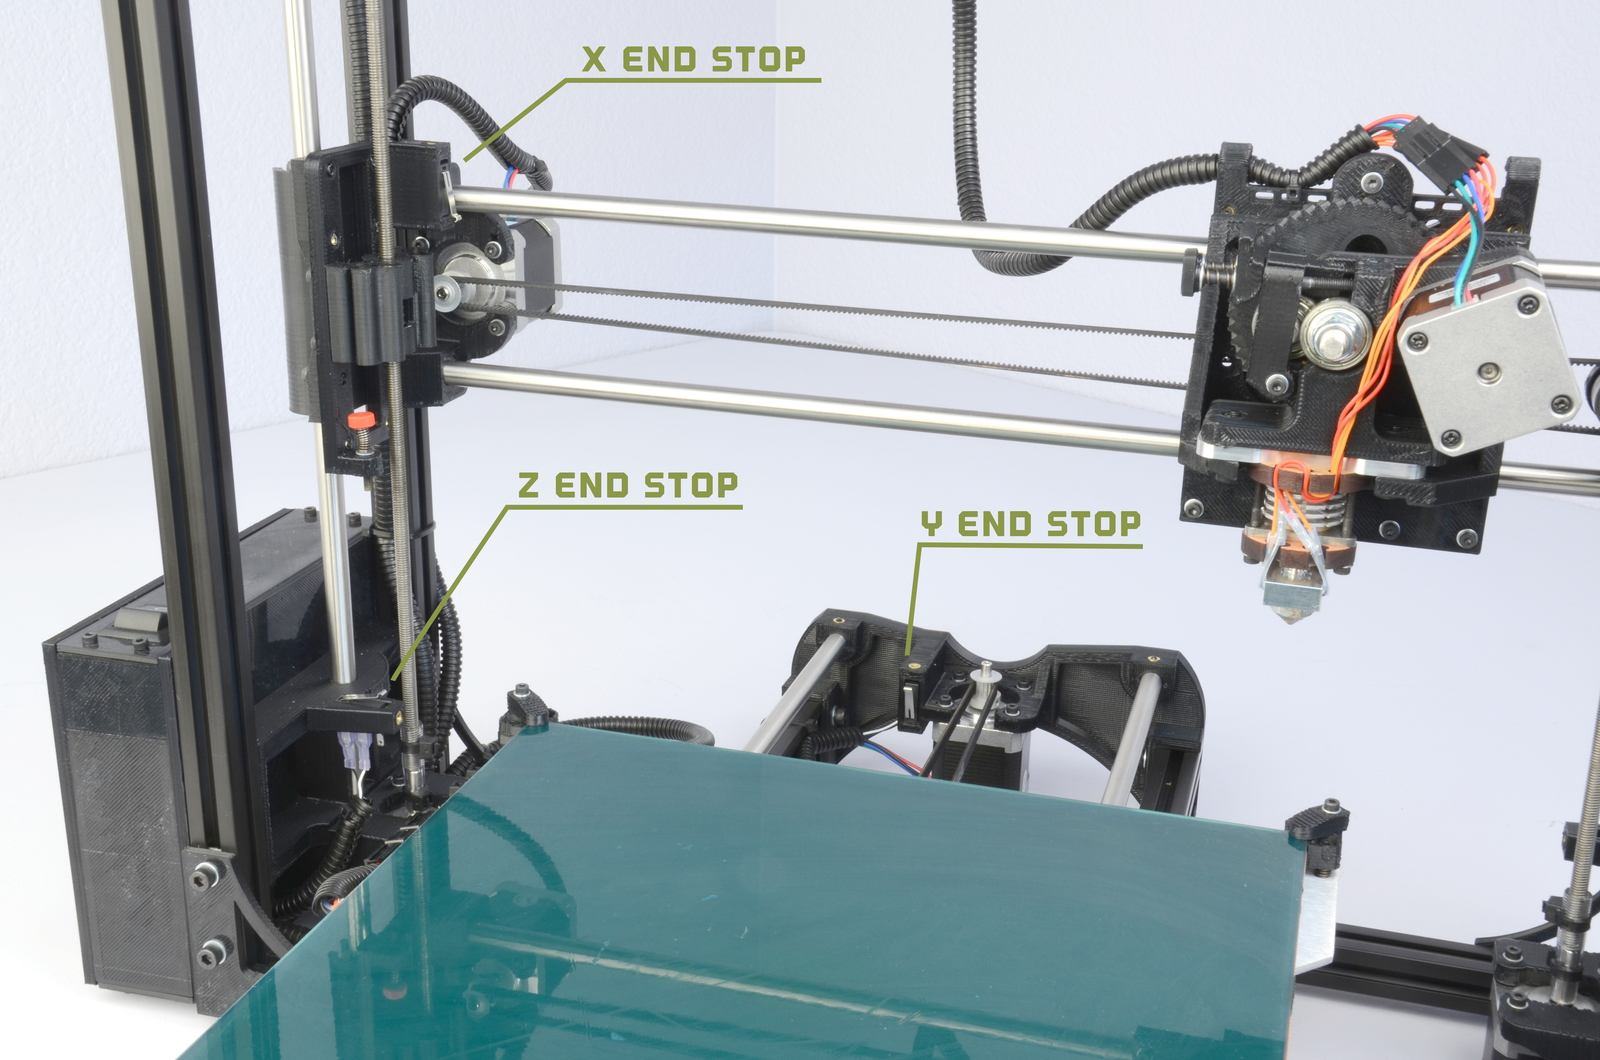
\includegraphics[keepaspectratio=true,angle=0,height=0.4\textheight,width=1.0\textwidth]{end_stop_switches.JPG}
\caption{End stop locations}
\label{fig:endstops}
\end{figure}

\end{enumerate}
